%!TEX spellcheck
%%%%%%%%%%%%%%%%%%%%%%%%%%%%%%%%%%%%%%%%%
% Beamer Presentation
% LaTeX Template
% Version 2.0 (March 8, 2022)
%
% This template originates from:
% https://www.LaTeXTemplates.com
%
% Author:
% Vel (vel@latextemplates.com)
%
% License:
% CC BY-NC-SA 4.0 (https://creativecommons.org/licenses/by-nc-sa/4.0/)
%
%%%%%%%%%%%%%%%%%%%%%%%%%%%%%%%%%%%%%%%%%

%----------------------------------------------------------------------------------------
%	PACKAGES AND OTHER DOCUMENT CONFIGURATIONS
%----------------------------------------------------------------------------------------

\documentclass[
	11pt, % Set the default font size, options include: 8pt, 9pt, 10pt, 11pt, 12pt, 14pt, 17pt, 20pt
	%t, % Uncomment to vertically align all slide content to the top of the slide, rather than the default centered
	%aspectratio=169, % Uncomment to set the aspect ratio to a 16:9 ratio which matches the aspect ratio of 1080p and 4K screens and projectors
	% handout,
]{beamer}

\graphicspath{{Images/}{./}} % Specifies where to look for included images (trailing slash required)

\usepackage{booktabs} % Allows the use of \toprule, \midrule and \bottomrule for better rules in tables

%----------------------------------------------------------------------------------------
%	SELECT LAYOUT THEME
%----------------------------------------------------------------------------------------

% Beamer comes with a number of default layout themes which change the colors and layouts of slides. Below is a list of all themes available, uncomment each in turn to see what they look like.

%\usetheme{default}
%\usetheme{AnnArbor}
%\usetheme{Antibes}
%\usetheme{Bergen}
%\usetheme{Berkeley}
%\usetheme{Berlin}
%\usetheme{Boadilla}
%\usetheme{CambridgeUS}
%\usetheme{Copenhagen}
%\usetheme{Darmstadt}
%\usetheme{Dresden}
%\usetheme{Frankfurt}
%\usetheme{Goettingen}
%\usetheme{Hannover}
%\usetheme{Ilmenau}
%\usetheme{JuanLesPins}
%\usetheme{Luebeck}
\usetheme{Madrid}
%\usetheme{Malmoe}
%\usetheme{Marburg}
%\usetheme{Montpellier}
%\usetheme{PaloAlto}
%\usetheme{Pittsburgh}
%\usetheme{Rochester}
%\usetheme{Singapore}
%\usetheme{Szeged}
%\usetheme{Warsaw}

%----------------------------------------------------------------------------------------
%	SELECT COLOR THEME
%----------------------------------------------------------------------------------------

% Beamer comes with a number of color themes that can be applied to any layout theme to change its colors. Uncomment each of these in turn to see how they change the colors of your selected layout theme.

%\usecolortheme{albatross}
%\usecolortheme{beaver}
%\usecolortheme{beetle}
%\usecolortheme{crane}
%\usecolortheme{dolphin}
%\usecolortheme{dove}
%\usecolortheme{fly}
%\usecolortheme{lily}
%\usecolortheme{monarca}
%\usecolortheme{seagull}
%\usecolortheme{seahorse}
%\usecolortheme{spruce}
%\usecolortheme{whale}
%\usecolortheme{wolverine}

%----------------------------------------------------------------------------------------
%	SELECT FONT THEME & FONTS
%----------------------------------------------------------------------------------------

% Beamer comes with several font themes to easily change the fonts used in various parts of the presentation. Review the comments beside each one to decide if you would like to use it. Note that additional options can be specified for several of these font themes, consult the beamer documentation for more information.

\usefonttheme{default} % Typeset using the default sans serif font
%\usefonttheme{serif} % Typeset using the default serif font (make sure a sans font isn't being set as the default font if you use this option!)
%\usefonttheme{structurebold} % Typeset important structure text (titles, headlines, footlines, sidebar, etc) in bold
%\usefonttheme{structureitalicserif} % Typeset important structure text (titles, headlines, footlines, sidebar, etc) in italic serif
%\usefonttheme{structuresmallcapsserif} % Typeset important structure text (titles, headlines, footlines, sidebar, etc) in small caps serif

%------------------------------------------------

%\usepackage{mathptmx} % Use the Times font for serif text
\usepackage{palatino} % Use the Palatino font for serif text
\usepackage{hyperref}
%\usepackage{helvet} % Use the Helvetica font for sans serif text
\usepackage[default]{opensans} % Use the Open Sans font for sans serif text
%\usepackage[default]{FiraSans} % Use the Fira Sans font for sans serif text
%\usepackage[default]{lato} % Use the Lato font for sans serif text
\usepackage{ctex}
\usepackage{siunitx}
\usepackage{tabularx}
\usepackage{umoline}
\usepackage{fourier}
%----------------------------------------------------------------------------------------
%	SELECT INNER THEME
%----------------------------------------------------------------------------------------

% Inner themes change the styling of internal slide elements, for example: bullet points, blocks, bibliography entries, title pages, theorems, etc. Uncomment each theme in turn to see what changes it makes to your presentation.

%\useinnertheme{default}
\useinnertheme{circles}
%\useinnertheme{rectangles}
%\useinnertheme{rounded}
%\useinnertheme{inmargin}

%----------------------------------------------------------------------------------------
%	SELECT OUTER THEME
%----------------------------------------------------------------------------------------

% Outer themes change the overall layout of slides, such as: header and footer lines, sidebars and slide titles. Uncomment each theme in turn to see what changes it makes to your presentation.

%\useoutertheme{default}
%\useoutertheme{infolines}
%\useoutertheme{miniframes}
%\useoutertheme{smoothbars}
%\useoutertheme{sidebar}
%\useoutertheme{split}
%\useoutertheme{shadow}
%\useoutertheme{tree}
%\useoutertheme{smoothtree}

%\setbeamertemplate{footline} % Uncomment this line to remove the footer line in all slides
%\setbeamertemplate{footline}[page number] % Uncomment this line to replace the footer line in all slides with a simple slide count

%\setbeamertemplate{navigation symbols}{} % Uncomment this line to remove the navigation symbols from the bottom of all slides

%----------------------------------------------------------------------------------------
%	PRESENTATION INFORMATION
%----------------------------------------------------------------------------------------

\title[Data Analysis]{Data Analysis} % The short title in the optional parameter appears at the bottom of every slide, the full title in the main parameter is only on the title page

\subtitle{数据分析} % Presentation subtitle, remove this command if a subtitle isn't required

\author[张凡]{张凡} % Presenter name(s), the optional parameter can contain a shortened version to appear on the bottom of every slide, while the main parameter will appear on the title slide

\institute[XDF]{新东方国际教育 \\ \smallskip \textit{zhangfan@xdf.cn}} % Your institution, the optional parameter can be used for the institution shorthand and will appear on the bottom of every slide after author names, while the required parameter is used on the title slide and can include your email address or additional information on separate lines

\date[\today]{GRE 冲分班数学 \\ \today} % Presentation date or conference/meeting name, the optional parameter can contain a shortened version to appear on the bottom of every slide, while the required parameter value is output to the title slide

%----------------------------------------------------------------------------------------


%----------------------------------------------------------------------------------------
%	Section Slide
%----------------------------------------------------------------------------------------
\AtBeginSection[]{
  \begin{frame}
  \vfill
  \centering
  \begin{beamercolorbox}[sep=8pt,center,shadow=true,rounded=true]{title}
    \usebeamerfont{title}\insertsectionhead\par%
  \end{beamercolorbox}
  \vfill
  \end{frame}

%----------------------------------------------------------------------------------------
%	TABLE OF CONTENTS SLIDE OF THE CURRENT SECTION
%----------------------------------------------------------------------------------------
	\begin{frame}
		\frametitle{Presentation Overview for \secname} % Slide title, remove this command for no title
		\tableofcontents[currentsection, hideothersubsections, sectionstyle=show/show]
	\end{frame}
  }

%----------------------------------------------------------------------------------------

\AtBeginSubsection[]{
  \begin{frame}
  \vfill
  \centering
    \usebeamerfont{title}\insertsubsectionhead\par%
  \vfill
  \end{frame}
}
%----------------------------------------------------------------------------------------


\begin{document}

%----------------------------------------------------------------------------------------
%	TITLE SLIDE
%----------------------------------------------------------------------------------------

\begin{frame}
	\titlepage % Output the title slide, automatically created using the text entered in the PRESENTATION INFORMATION block above
\end{frame}



%----------------------------------------------------------------------------------------
%	PRESENTATION BODY SLIDES
%---------------------------------------------------------------------------------------

\section{Counting Methods}

%------------------------------------------------

\subsection{Lists}
\begin{frame}
	\frametitle{Lists} % Slide title, remove this command for no title
	\framesubtitle{列表:有顺序可重复}
	\begin{definition}
		\begin{itemize}
			\item In a list, the members are ordered—that is, rearranging the members of a list makes it a different list.
			\item Elements can be repeated in a list and the repetitions matter.
		\end{itemize}
	\end{definition}
	\begin{example}
		1, 2, 3 and 2, 3, 1 and 1, 1, 2, 3 are all different list. 
	\end{example}
\end{frame}

%------------------------------------------------

\subsection{Sets}
\begin{frame}
	\frametitle{Sets} % Slide title, remove this command for no title
	\framesubtitle{集合:无顺序不可重复}
	\begin{definition}
		\begin{itemize}
			\item In a set, repetitions are
not counted as additional elements.
			\item the order of the elements does not
matter.
		\end{itemize}
	\end{definition}
	\begin{example}
		\{1, 2, 3\} and \{2, 3, 1\} and \{1, 1, 2, 3\} are the same set. 
	\end{example}
\end{frame}

%------------------------------------------------

\begin{frame}
	\frametitle{Subsets} % Slide title, remove this command for no title
	\framesubtitle{空集是任意集合的子集}
	\begin{definition}
	If A and B are sets and all of the
members of A are also members of B, then A is a subset of B. By convention, $\emptyset$ is a subset of
every set.
	\end{definition}
	\begin{example}
		\{2, 8\} is a subset of \{0, 2, 4, 6, 8\}.
	\end{example}

	\begin{theorem}
		If a set has n elements, then the number of subset of the given set is $2^n$
	\end{theorem}
	\alert{We will prove the above theorem by induction when we talk about Combinations.}
\end{frame}

%------------------------------------------------
%TO-DO: intersection, mutual exclusive

\begin{frame}
	\frametitle{The Intersection of Sets} % Slide title, remove this command for no title
	\framesubtitle{交集}
	\begin{definition}
If S and T are sets, then the
intersection of S and T is the set of all elements that are in both S and T and
is denoted by $S \cap	T$
	\end{definition}
	\begin{example}
		The intersection of set \{1, 2, 3, 5\} and \{2, 3, 5, 6\} is \{2, 3, 5\}.
	\end{example}
\end{frame}

%------------------------------------------------
\begin{frame}
	\frametitle{Subsets, Intersection and Disjoint} % Slide title, remove this command for no title
	\framesubtitle{子集, 交集和互斥}
	\begin{definition}
If sets S and T have no
elements in common, they are called \alert{disjoint} or \alert{mutually exclusive}.
	\end{definition}

		\begin{figure}
		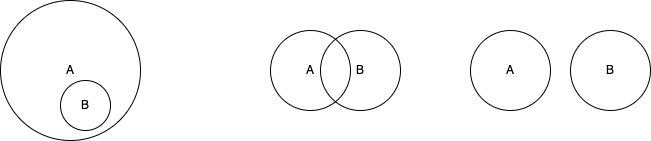
\includegraphics[width=\linewidth]{Disjoint.png}
		\caption{$A\cap B = B$ (left); $B\cap A$ (center); $B \cap A = \emptyset $(right).}
	\end{figure}
\end{frame}

%------------------------------------------------

\begin{frame}
	\frametitle{Have a try!}
If there are 200 millions people who have at least one cat in US and 300 millions people who have at least one dog, what is range for the number of people who have at least one cat \alert{and} at least one dog?


\pause
\bigskip\bigskip\bigskip\bigskip
Answer \textbf{$$0 \leq x \leq 200$$}
\end{frame}


%------------------------------------------------

\begin{frame}
	\frametitle{Union of Sets} % Slide title, remove this command for no title
	\framesubtitle{并集}
	\begin{definition}
The \alert{union} of S and T is the set of all elements that are
in either S or T or both and is denoted by $$S\cup	T$$.
	\end{definition}

	\alert{Sets don't allow repeatable elements.}
	\begin{example}
		The intersection of set \{1, 2, 3, 5\} and \{2, 3, 5, 6\} is \{1, 2, 3, 5, 6\}.
	\end{example}	
\end{frame}

%------------------------------------------------

\begin{frame}
	\frametitle{Inclusion-Exclusion Principle} % Slide title, remove this command for no title
	\framesubtitle{容斥原理}
	\begin{theorem}
	\begin{equation}
		\mid A \cup B \mid = \mid A \mid + \mid B \mid - \mid A \cap B \mid 
	\end{equation}
	\end{theorem}

	\begin{figure}
		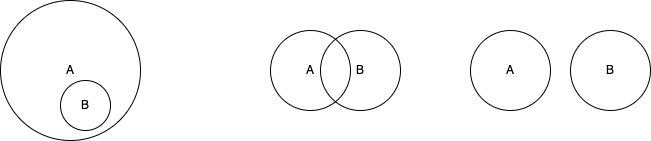
\includegraphics[width=\linewidth]{Disjoint.png}
		\caption{
			$\mid A \cup B \mid = \mid A \mid $(left); $\mid A \cup B \mid = \mid A \mid + \mid B \mid - \mid A \cap B \mid $ (center); $\mid A \cup B \mid = \mid A \mid + \mid B \mid$ (right).}
	\end{figure}

\end{frame}

%------------------------------------------------


\begin{frame}
	\frametitle{Have a try!}
If there are 200 millions people who have at least one cat in US and 300 millions people who have at least one dog, what is range for the number of people who have at least one cat \alert{or} at least one dog?


\pause
\bigskip\bigskip\bigskip\bigskip
Answer \textbf{$$300 \leq x \leq 500$$}
\end{frame}


%------------------------------------------------

\subsection{Addition Principle}

%------------------------------------------------

\begin{frame}
	\frametitle{A Vanilla Question} % Slide title, remove this command for no title
	\framesubtitle{互斥相加}
			In the Happy Meal of McDonald's, You can either have a hamburger or Chicken McNuggets but not both. There are 2 flavors for the hamburger and 3 flavors for the Chicken McNuggets. How many options do you have for the Happy Meal?\\
			\pause
			\begin{figure}
				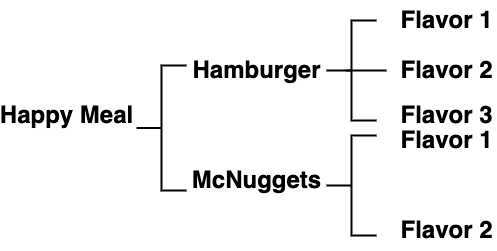
\includegraphics[width=0.5\linewidth]{Addition_Vanilla.png}
			\end{figure}
			\bigskip
			\pause
			Answer \textbf{$3 + 2 = 5$}
\end{frame}


%------------------------------------------------

\begin{frame}
	\frametitle{Addition Principle} % Slide title, remove this command for no title
	\framesubtitle{加法原则}
	\begin{definition}
		\begin{itemize}
      \item if we have k number of ways of doing something A and k number of ways of doing another thing B
      \item and if \alert{we can not do both A and B at the same time}. ($A \cap B = \emptyset$)
		\end{itemize}
				Then, there are A + B ways to choose one of the actions.
	\end{definition}
	\textbf{Have a try!}\\
	 How many different are there for the one-character code name for an agent in \emph{Men In Black}, which can be a digit or a letter?\\ \pause
	 Answer \textbf{24 +  10 = 34}
	
\end{frame}

%------------------------------------------------

\subsection{Multiplication Principle}

%------------------------------------------------

\begin{frame}
	\frametitle{A Vanilla Question} % Slide title, remove this command for no title
	\framesubtitle{每个branch的subbranch数量相同相乘}
						In the Happy Meal of McDonald's, You can either have a hamburger or Chicken McNuggets but not both. There are 2 flavors for the hamburger and 3 flavors for the Chicken McNuggets. You can choose your beverage between Coca Cola and Milk. How many options do you have for the Happy Meal?\\
			\pause

	\begin{columns}[t] 
		\begin{column}{0.6\textwidth} % Left column width 
		\pause
			\begin{figure}
				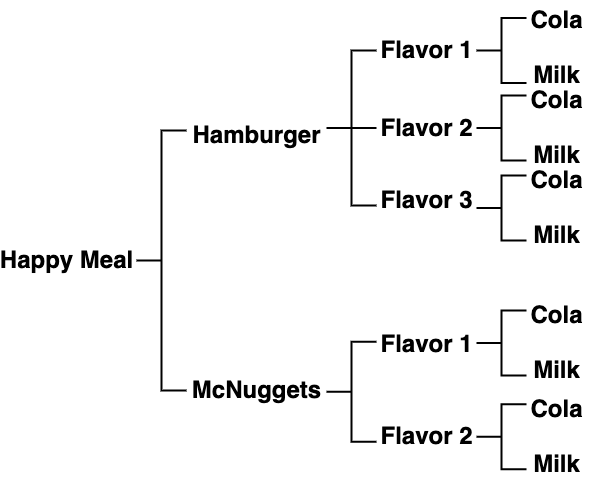
\includegraphics[width=0.8\linewidth]{Multiplication_Vanilla.png}
			\end{figure}
		\end{column}
		\begin{column}{0.3\textwidth} % Right column width

			\pause
			Answer \textbf{$(3 + 2)\times 2 = 10$}
		\end{column}
	\end{columns}

\end{frame}


%------------------------------------------------

\begin{frame}
	\frametitle{Multiplication Principle} % Slide title, remove this command for no title
	\framesubtitle{乘法原则}
	\begin{definition}
		\begin{itemize}
			\item Suppose there are two choices to be made sequentially.
			\item Suppose also that there are $k$ different possibilities for the first choice and $m$ different possibilities for the second choice for each possibilities of the first choice. 
		\end{itemize}
				Then, \alert{under those conditions}, there are $km$ different possibilities for the pair of choices.
	\end{definition}
	\begin{example}
	For a 6 digit Bank PIN, there could be $10^6$ different passwords. 
	\end{example}
\end{frame}

%------------------------------------------------

\begin{frame}
	\frametitle{Have A Try} % Slide title, remove this command for no title
	\framesubtitle{ 不用画树直接算}
	What if a 6 digit Bank PIN can not start or end with 0?

	\bigskip \bigskip
	Answer \textbf{$9 \cdot 10^4 \cdot 9$}
	\alert{What if the digit are not independent?}
\end{frame}

%------------------------------------------------



\begin{frame}
	\frametitle{Demo}
	\framesubtitle{难题演示}
\textbf{GMAT-OG} In a meeting of 3 representatives from each of 6 different companies, each person
shook hands with every person not from his or her own company. If the representatives did not shake hands with people from their own company, how many handshakes took place?
	\begin{columns}[t] 
		\begin{column}{0.5\textwidth} % Left column width
			\begin{enumerate}[A]
				\item 45
			  \item 135
			  \item 144
			  \item 270
			  \item 288
			\end{enumerate}
		\end{column}
		\begin{column}{0.5\textwidth} % Right column width
			\begin{figure}
				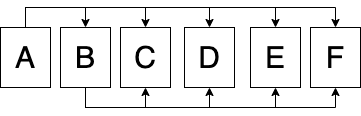
\includegraphics[width=0.5\linewidth]{Handshakes.png}
				\caption{Handshakes for Company A should be $3\times15 = 45$;Handshakes for Company B should be $3\times12 = 36$.}
			\end{figure}		
			$3 \times 15 + 3 \times 12 + 3\times 9 + 3 \times 6 + 3\times3 = 135$
			\pause
      Answer \textbf{B} 135 \pause 
		\end{column}
	\end{columns}
\end{frame}

%------------------------------------------------


\subsection{Permutations}

%------------------------------------------------

\begin{frame}
	\frametitle{A Vanilla Question} % Slide title, remove this command for no title
	\framesubtitle{排排坐的排法}
	\begin{columns}[t] 
		\begin{column}{0.3\textwidth} % Left column width
			How many kinds of different lists can be constructed 3 Students --- student A, student B and student C.  
		\end{column}
		\begin{column}{0.7\textwidth} % Right column width
		  \pause
			\begin{figure}
				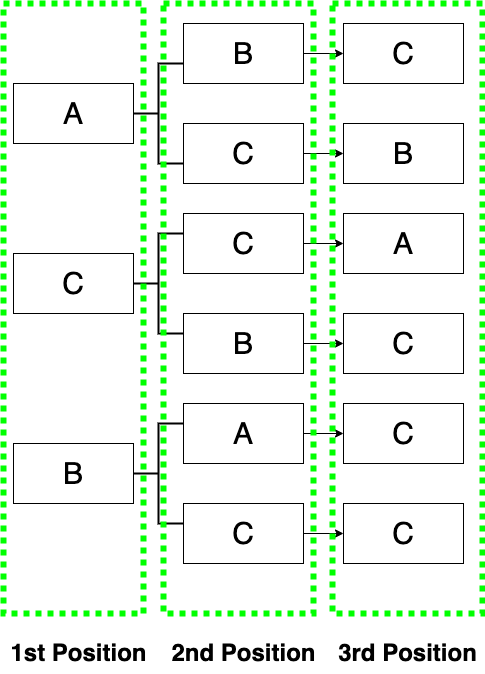
\includegraphics[width=0.5\linewidth]{Permutation3.png}
				\caption{6 Different Lists can be formed from 3 different students}
			\end{figure}
		\end{column}
	\end{columns}
\end{frame}


%------------------------------------------------

\begin{frame}
	\frametitle{A Vanilla Question} % Slide title, remove this command for no title
	\framesubtitle{排排坐的排法}
	\begin{columns}[t] 
		\begin{column}{0.3\textwidth} % Left column width
		   What about the 4 different students?\\
		   5 different students\\
		   6 different students\\
		   $\vdots$

		\end{column}
		\begin{column}{0.7\textwidth} % Right column width
		  \pause
		  \begin{equation*}
		  		  	4 \times 3 \times 2 \times 1 = 24 
		  \end{equation*}
		\end{column}
	\end{columns}
\end{frame}

%------------------------------------------------

\begin{frame}
	\frametitle{Permutation} % Slide title, remove this command for no title
	\framesubtitle{全排}
	\begin{definition}
		Suppose n objects are to be ordered from 1st to nth, then
 the number of ways the objects can be ordered is $n(n-1)(n-2)(n-3)\ldots1=n!$ 
	\end{definition}
\end{frame}

%------------------------------------------------

\begin{frame}
\frametitle{Have a try!}
\framesubtitle{把Bus Seats 编号}
\textbf{og-p463-1.7.16} Suppose that 10 students are going on a bus trip, and each
of the students will be assigned to one of the 10 available seats. What is  the
number of possible different seating arrangements of the students on the
bus?


\bigskip
\pause
$10! = 10 \times 9 \times 8 \times 7 \ldots 1 = 3,628,800  $\\
\bigskip\pause
Answer \textbf{3,628,800} \pause 
\end{frame}

%------------------------------------------------

\begin{frame}
	\frametitle{Have a try!}
	\framesubtitle{}
A gardener wishes to plant 5 bushes in straight row. Each bush has flowers of a
different solid color (white, yellow, pink, red, and purple). How many ways can the
bushes be arranged so that middle bush is the one with red flowers?
	\begin{figure}
		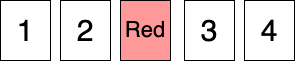
\includegraphics[width=0.3\linewidth]{Bushes.png}
		\caption{There are 4 vacancy.}
	\end{figure}
\begin{equation*}
	^5P_4 =\frac{5!}{(5-4)!} = 5! = 120
\end{equation*}
\bigskip
\pause
Answer \textbf{$120$}
\bigskip

\end{frame}

%------------------------------------------------

\begin{frame}
	\frametitle{A Real QR Problem!}
	\framesubtitle{}
	\begin{figure}
		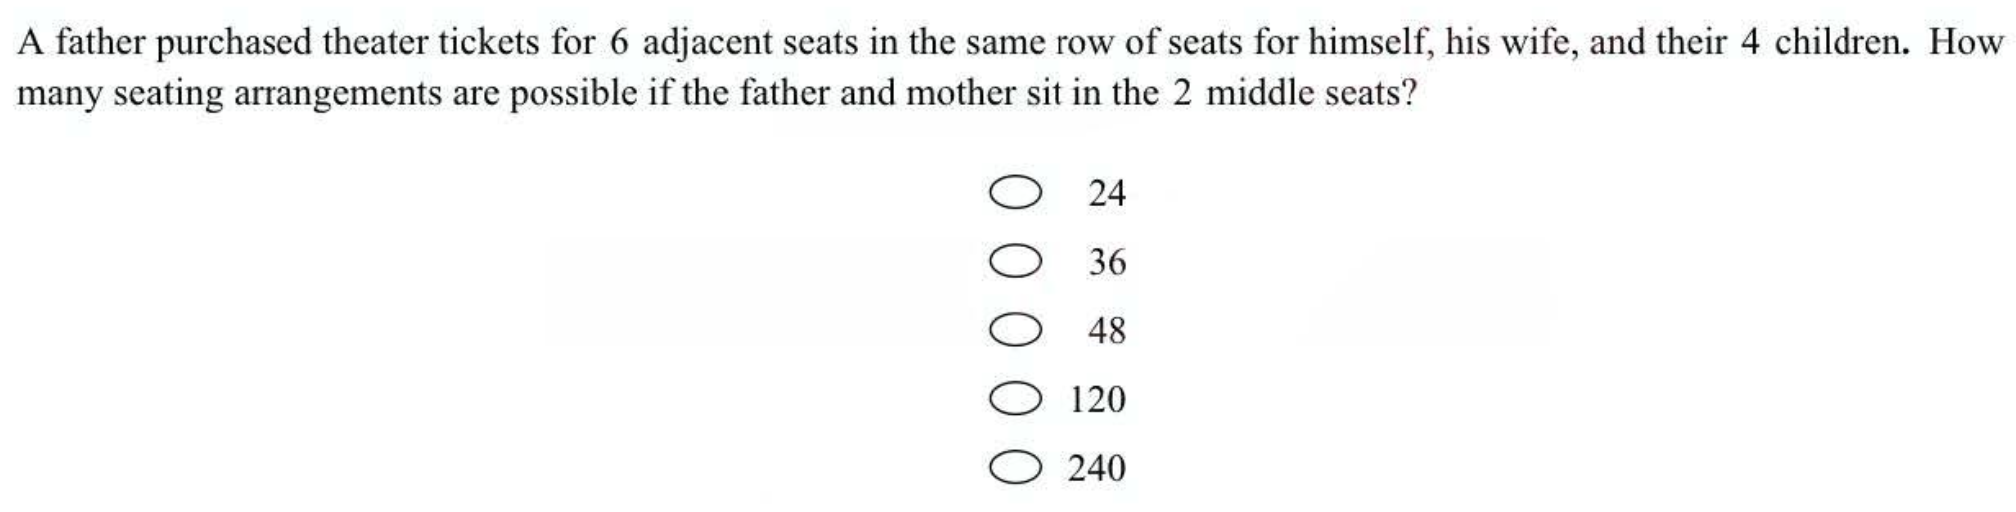
\includegraphics[width=\linewidth]{K-Permutation_Example_Question.png}
		\caption{8-Sec3-8}
	\end{figure}
	\pause
$Children's\ Permutation= 4! =24$\\
$Parents'\ Permutation= 2! =2$\\
$Possible Arrangements= (Children's\ Permutation) \cdot (Parents'\ Permutation) =4! \cdot 2!=48$\\

\pause
\bigskip
Answer \textbf{C}  48
\end{frame}


%------------------------------------------------

\subsection{K-Permutation}

%------------------------------------------------
 
 \begin{frame}
	\frametitle{A Vanilla Question} % Slide title, remove this command for no title
	\framesubtitle{选部分人排排坐的排法}
	 Suppose that there are 8 students and 5 students are selected going on a bus trip, and each
of the students will be assigned to one of the 5 available seats. What is  the
number of possible different seating arrangements of the students on the
bus?

	\begin{figure}
		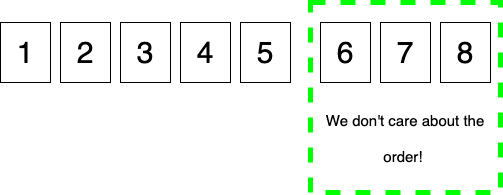
\includegraphics[width=0.5\linewidth]{K_permutation.png}
		\caption{The order about the final 3 students is irrelevant.}
	\end{figure}
	\begin{equation}
		\frac{8!}{3!} = \frac{8\times7\times6\cdots\times1}{3\times2\times1} = 6,720
	\end{equation}
\end{frame}

%------------------------------------------------

\begin{frame}
	\frametitle{K-Permutation} % Slide title, remove this command for no title
	\framesubtitle{K-全排}
	\begin{definition}
		Suppose that k objects will be selected from a set of n
objects, where , and the k objects will be placed in order from 1st to
kth, the number of ways to select and order k objects from a set of n objects is \\
\begin{equation*}
	^nP_k =\frac{n!}{(n-k)!}
\end{equation*}
	\end{definition}
\end{frame}

%------------------------------------------------


\begin{frame}
	\frametitle{Demo: K-Permutation} % Slide title, remove this command for no title
	\framesubtitle{难题演示}
	How many distinguished way to arrange the word “ORDER” if there are at least
	two letters between two “R”s?

		\begin{columns}[t] 
			\begin{column}{0.5\textwidth} % Left column width
				\begin{figure}
					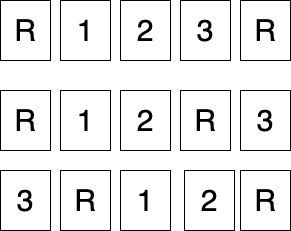
\includegraphics[width=0.8\linewidth]{ORDER.png}
					\caption{Three possible arrangements with blanks to fill}
				\end{figure}
			\end{column}
			\begin{column}{0.5\textwidth} % Right column width
				\begin{equation*}
					\begin{aligned}
						&^3P_3+ ^3P_2 \cdot 2 \\
						&=3! + \frac{3!}{2!} \cdot 2 \\
						&=18
					\end{aligned}
				\end{equation*}
			\end{column}
		\end{columns}
\end{frame}

%------------------------------------------------




\subsection{Combinations}

%------------------------------------------------
 
 \begin{frame}
	\frametitle{A Vanilla Question} % Slide title, remove this command for no title
	\framesubtitle{选部分人不讲顺序的排法}
	 Suppose that there are 8 students and 5 students are selected going on a bus trip. What is  the
number of possible combinations of the students on the for the bus trip?

	\begin{figure}
		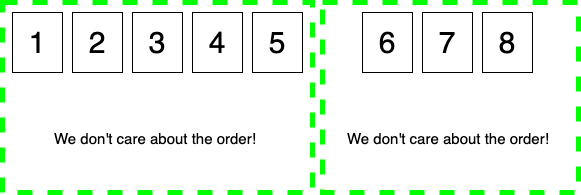
\includegraphics[width=0.5\linewidth]{Combination_8_5.png}
		\caption{The order about the  3 students abandoned and the 5 students chosen is irrelevant.}
	\end{figure}
	\begin{equation}
		\frac{8!}{5! 3!} = \frac{8\times7\times6\cdots\times1}{(5\times4\times3\times2\times1)(3\times2\times1)} = 56
	\end{equation}
\end{frame}

%------------------------------------------------

\begin{frame}
	\frametitle{Combinations} % Slide title, remove this command for no title
	\framesubtitle{n选k,不讲顺序}
	\begin{definition}
		Suppose that k objects will be chosen from a set of n
		objects, where , but that the k objects will not be put in order. The
		 the number of combinations of n objects taken k at a time and is \\
		\begin{equation*}
		  ^nC_k =\frac{n!}{k!(n-k)!}
		\end{equation*}
	\end{definition}

	\begin{proof}
		\begin{equation*}
			\begin{aligned}
				&(number\ of\ ways\ to\ select\ without\ order)\ \times\ (number\ of\ ways\ to\ order)\\ =
&(number\ of\ ways\ to\ select\ with\ order)\\
&(number\ of\ ways\ to\ select\ without\ order) =\\
&\frac{(number\ of\ ways\ to\ select\ with\ order)}{(number\ of\ ways\ to\ order)}
			\end{aligned}
		\end{equation*}
	\end{proof}
\end{frame}

%------------------------------------------------

\begin{frame}
	\frametitle{Have a try!}
	\framesubtitle{}
Suppose you want to select a 3-person committee from a
group of 9 students. How many ways are there to do this?
\pause
\begin{equation*}
	^9C_3 =\frac{9!}{3!6!} = 84
\end{equation*}
\bigskip
\pause
Answer \textbf{$84$} 
\end{frame}

%------------------------------------------------

\begin{frame}
	\frametitle{Rules of Combination}
	\framesubtitle{快速计算规则}
	\begin{itemize}
		\item $^nC_0=1$
		\item $^nC_1=n$ 
		\item $^nC_r = ^nC_{n-r}$ 
	\end{itemize}
\end{frame}


%------------------------------------------------

\begin{frame}
	\frametitle{Binomial Expansion}
	\framesubtitle{二项式展开}
	\begin{theorem}
			\begin{equation*}
			\begin{aligned}
				(x + y)^n = ^nC_0x^0 y^n + ^nC_1x y^{n-1} + ^nC_2x^2 y^{n-2} + \cdots + ^nC_0x^n y^{0}\\
			\end{aligned}		
			\end{equation*}		
	\end{theorem}
	\begin{corollary}
		Make $x=y =1$,
			\begin{equation*}
			\begin{aligned}
				2^n = ^nC_0+ ^nC_1 + ^nC_2 + \cdots + ^nC_0\\
			\end{aligned}		
			\end{equation*}		
	\end{corollary}
\end{frame}


%------------------------------------------------


\begin{frame}
	\frametitle{Proof by Induction: $2^n$ different subsets for a set of n elements }
	\framesubtitle{$2^n$ 不同子集}
		\begin{theorem}
		If a set has n elements, then the number of subset of the given set is $2^n$
	\end{theorem}

	\begin{proof}
		Base Case (n=0): When $n=0$, there is only $2^0 =1$ subset for $\emptyset$, namely itself.\\
		Inductive Step $(n \rightarrow n + 1)$: \\
		When we add a new element e to the original n-element set, the subset either contains the new element e or not.\\
		There are $2^n$ subsets which do not contain the new element  e.\\
		There are $2^n = ^nC_0+ ^nC_1 + ^nC_2 + \cdots + ^nC_0$ elements who do contains the new element e.\\
		There are $2^{n+1}$ subsets for a set with $(n + 1)$ elements.\\
	\end{proof}
\end{frame}


%------------------------------------------------

\begin{frame}
	\frametitle{Have a try!}
	\framesubtitle{}
There are five points on line $l_1$ and four points on $l_2$. If $l_1$ and $l_2$ are parallel, how
many different triangles can be constructed based on these nine points?
  \pause
	\begin{figure}
		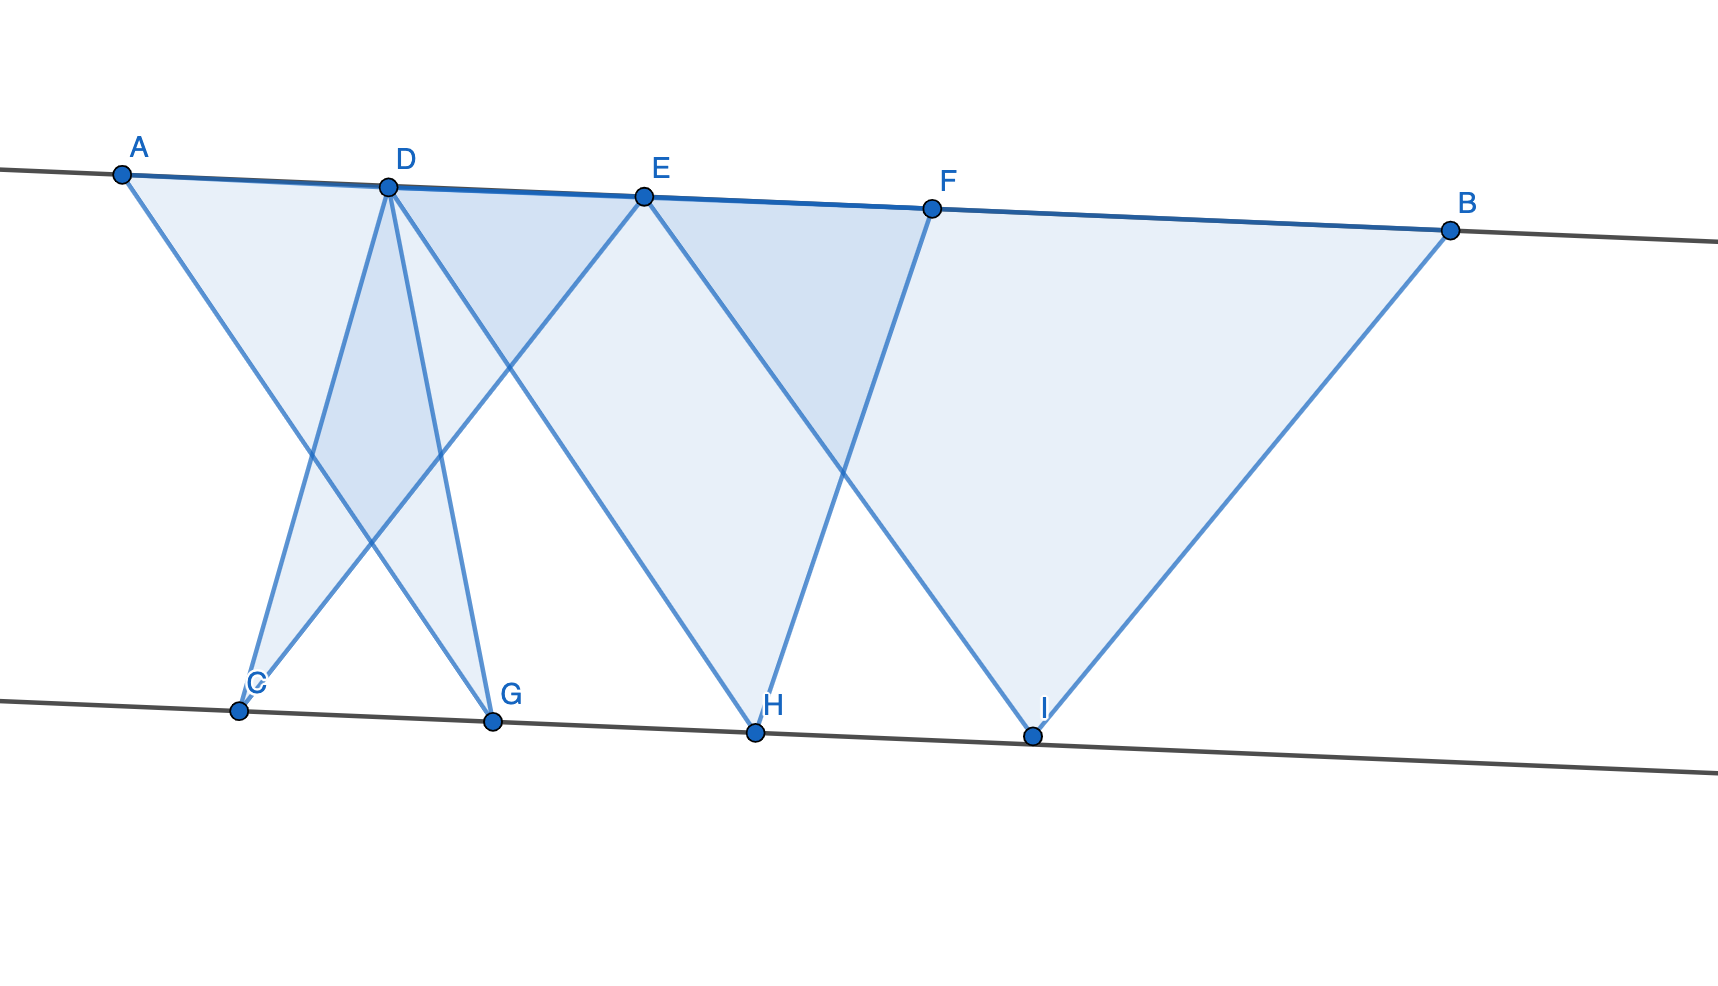
\includegraphics[width=0.5\linewidth]{Triangles_Combinations.png}
	\end{figure}

	$$^2C_5 \cdot ^1C_4 + ^1C_5 \cdot^2C_4 = 70$$  
	\bigskip
	\pause
Answer \textbf{$70$} 
\end{frame}

%------------------------------------------------
\begin{frame}
	\frametitle{Have a try!}
	\framesubtitle{}
A man walks to his home from his current location on the rectangular grid shown. If
he may choose to walk north or east at any corner, but may never moves south or
west. How many different paths can the man take to get home?
	\begin{figure}
		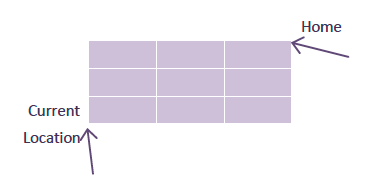
\includegraphics[width=0.5\linewidth]{Man_Walk.png}
	\end{figure}
\bigskip
\pause
Answer \textbf{$^6 C_3 = 20$}
\bigskip
\end{frame}

%------------------------------------------------



\begin{frame}
	\frametitle{Demo}
	\framesubtitle{反其道而行之:用总数去减}
\textbf{GMAT-鸡精} In a certain class of 20 students with different initials of surname, the roster is arranged by the order of initial of surnames. If three students are selected to join a
seminar, how many different ways to select them whose initial of surnames are not
near to each other?
	\begin{columns}[t] 
		\begin{column}{0.3\textwidth} % Left column width
				\begin{figure}
				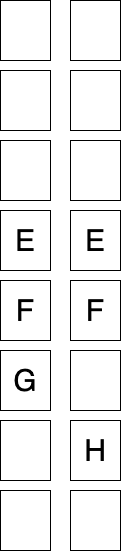
\includegraphics[width=0.2\linewidth]{Surnames.png}
				\caption{Two combinations that are not allowed.}
				\end{figure}		
		\end{column}
		\begin{column}{0.7\textwidth} % Right column width
		Case 1: Three consecutive initials\\
		$Combination_1 = 18$\\
		\bigskip
		Case 2: Only two consecutive initials \\
		Case 2-1: the two consecutive initials occupies the start or the end of the roster\\
		$Combination_{2-1} = 2 \times 17 = 34$\\
		Case 2-2: the two consecutive initials occupies neither the start nor the end of the roster\\
		$Combination_{2-2} = 17 \times 16 = 186$\\
		$\therefore ^3C_{20} - Combination_1 -Combination_{2-1} - Combination_{2-2} = 1140 - 18 - 34 - 186 = \textbf{902}$
		\end{column}
	\end{columns}
\end{frame}

%------------------------------------------------

\begin{frame}
	\frametitle{A Real QR Problem!}
	\framesubtitle{}
	\begin{figure}
		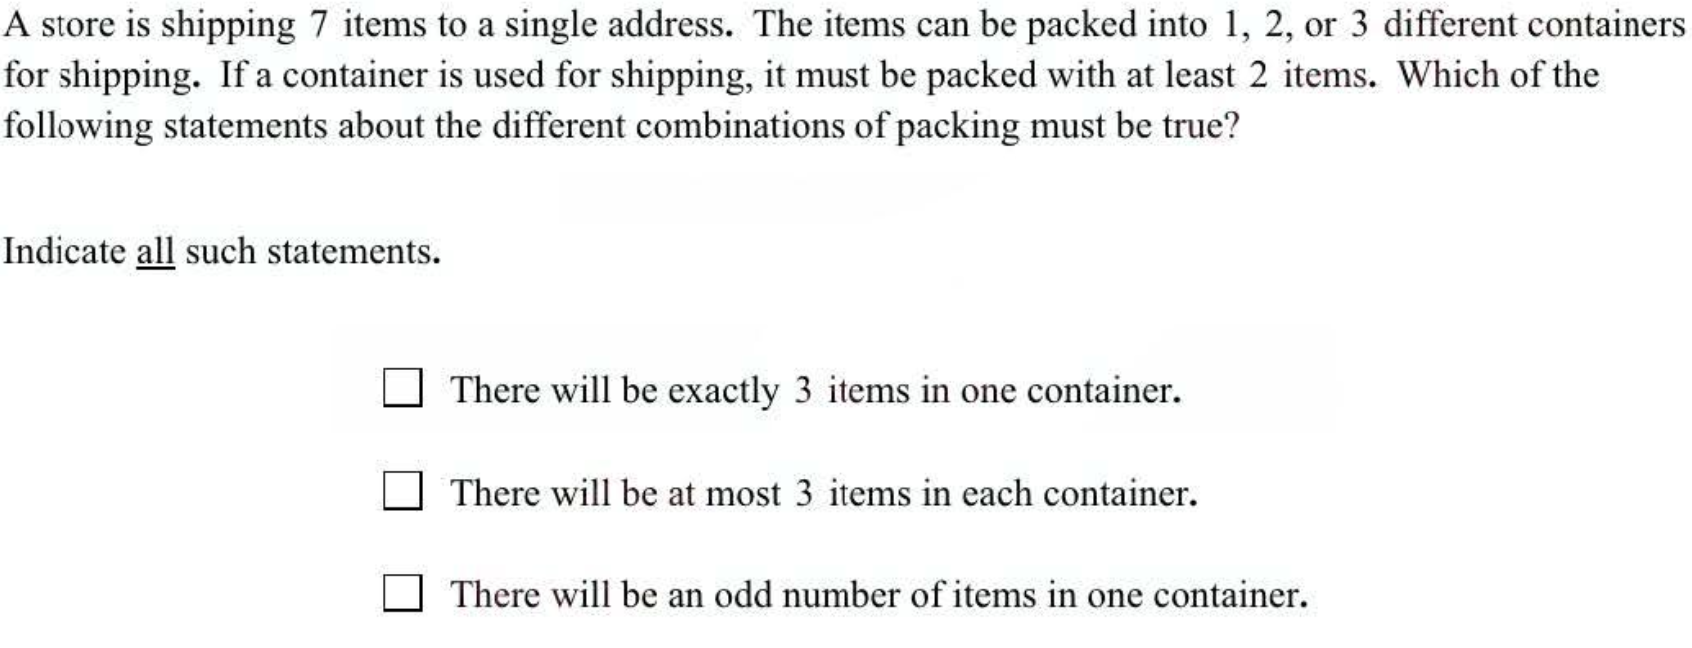
\includegraphics[width=\linewidth]{Combinations_Example_Question.png}
		\caption{9-Sec1-12}
	\end{figure}
	
\end{frame}

%------------------------------------------------

\begin{frame}
	\frametitle{A Real QR Problem!}
	\framesubtitle{}
	\pause
	\begin{figure}
		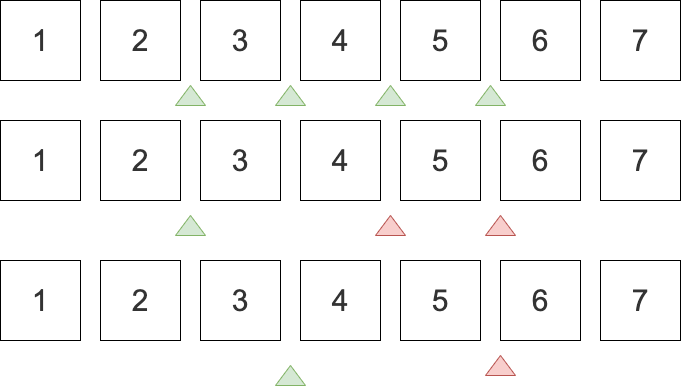
\includegraphics[width=0.5\linewidth]{Boxes.png}
		\caption{ 2 boxes (top); 3 boxes (center); 3 boxes(bottom).}
	\end{figure}
\pause
$ a  = 7; a + b = 7; a + b + c = 7.$
\pause
\bigskip
Answer \textbf{B } There will be an odd number of items in one container.
\end{frame}

%------------------------------------------------

\begin{frame}
	\frametitle{Have a try!}
	\framesubtitle{How many different combinations are there?}
	\begin{figure}
		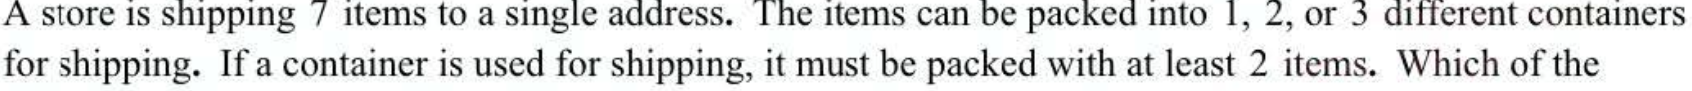
\includegraphics[width=\linewidth]{Combinations_Example_Question_1.png}
		\caption{9-Sec1-12}
	\end{figure}
		\begin{figure}
		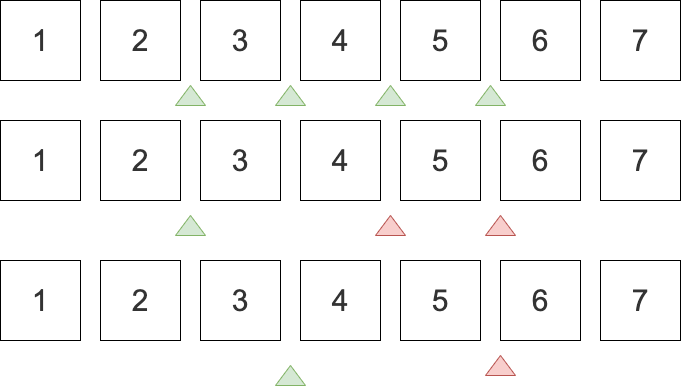
\includegraphics[width=0.5\linewidth]{Boxes.png}
	\end{figure}
\pause
	\pause
	Answer \textbf{$1\cdot ^3P_3+4\cdot ^3P_3+ 3\cdot ^3P_3 = 48$} \\
	\alert{The items are the same; But the containers are not.}
\end{frame}

%------------------------------------------------

\section{Probability}

%------------------------------------------------

\subsection{Events}
\begin{frame}
	\frametitle{Events}
	\framesubtitle{Events是outcomes的集合}
	
	\begin{definition}
		Any particular set of outcomes is called an \alert{event}.
	\end{definition}
	\begin{example}
		For a fair 6-sided dice, \\
		Event O: the number facing-up is odd.\\
		Equivalently, O = {1, 3, 5}
	\end{example}
\end{frame}

%------------------------------------------------

\begin{frame}
	\frametitle{Sample Space}
	\framesubtitle{包含所有的outcomes}
	
	\begin{definition}
		The set of
all possible outcomes of a random experiment is called the \alert{sample space}.
	\end{definition}
	\begin{example}
		For a fair 6-sided dice, the sample space is 	 \{1, 2, 3, 4, 5, 6\}\\
	\end{example}
\end{frame}

%------------------------------------------------


\begin{frame}
	\frametitle{Event A Or Event B Happens}
	\framesubtitle{A或B;A发生,B发生,或者AB都发生}
	\begin{definition}
	 $P(A or B) = P(A \cup B) = P(A)  + P(B) - P(A and B)$
	\end{definition}

	\begin{example}
		Event O: the number facing-up is odd.\\ O = \{1, 3, 5\}\\
		Event T: the number facing-up is a multiple of 3.\\ T = \{3, 6\}\\
		O or T = \{1, 3, 5, 6\}
	\end{example}
\end{frame}

%------------------------------------------------


\subsection{Mutually Inclusive Events}

%------------------------------------------------


\begin{frame}
	\frametitle{Mutually Exclusive Events}
	\framesubtitle{互斥事件无法同时发生}
	\begin{definition}
		\begin{itemize}
			\item Events that cannot occur at the same time are said to be mutually
exclusive.
      \item  Events that don't have a common outcome are said to be mutually
exclusive.
		\end{itemize}
	\end{definition}


	\begin{example}
		Event A: A card randomly selected from a pack is Diamonds K.\\
		A=\{Diamonds K\}\\
		Event B: A card randomly selected from a pack is Hearts.\\
		B = \{Hearts A, Hearts 2, $\cdots$, Heart K\}
	\end{example}
\end{frame}

%------------------------------------------------


\begin{frame}
	\frametitle{Event A Or Event B Happens when they are mutually exclusive}
	\framesubtitle{互斥事件的或:A发生,或者B发生}
	
	\begin{definition}
	 $P(A\ or\ B) = P(A \cup B) = P(A)  + P(B)$
	\end{definition}
	\begin{example}
		Event A: A card randomly selected from a pack is Diamonds K.\\
		A=\{Diamonds K\}\\
		Event B: A card randomly selected from a pack is Hearts.\\
		B = \{Hearts A, Hearts 2, $\cdots$, Heart K\}\\
		A or B = \{Diamonds K, Hearts A, Hearts 2, $\cdots$, Heart K\}
	\end{example}
\end{frame}

%------------------------------------------------

\subsection{Conditional Probability}

%------------------------------------------------

\begin{frame}
	\frametitle{Conditional Probability}
	\framesubtitle{条件概率:一定要找到分母}
	
	\begin{definition}
	 $$P(A\mid B) = \frac{P(A and B)}{P(B)}$$
	\end{definition}
	\begin{example}
		Event A: A card randomly selected from a pack is Hears K.\\
		A=\{Diamonds K\}\\
		Event B: A card randomly selected from a pack is Hearts.\\
		B = \{Hearts A, Hearts 2, $\cdots$, Heart K\}\\
		$P(A \mid B)  = \frac{1}{13}$
	\end{example}
	\alert{given that, suppose that, if, when}
\end{frame}

%------------------------------------------------

\begin{frame}
	\frametitle{A Real QR Problem!}
	\framesubtitle{}
	\begin{figure}
		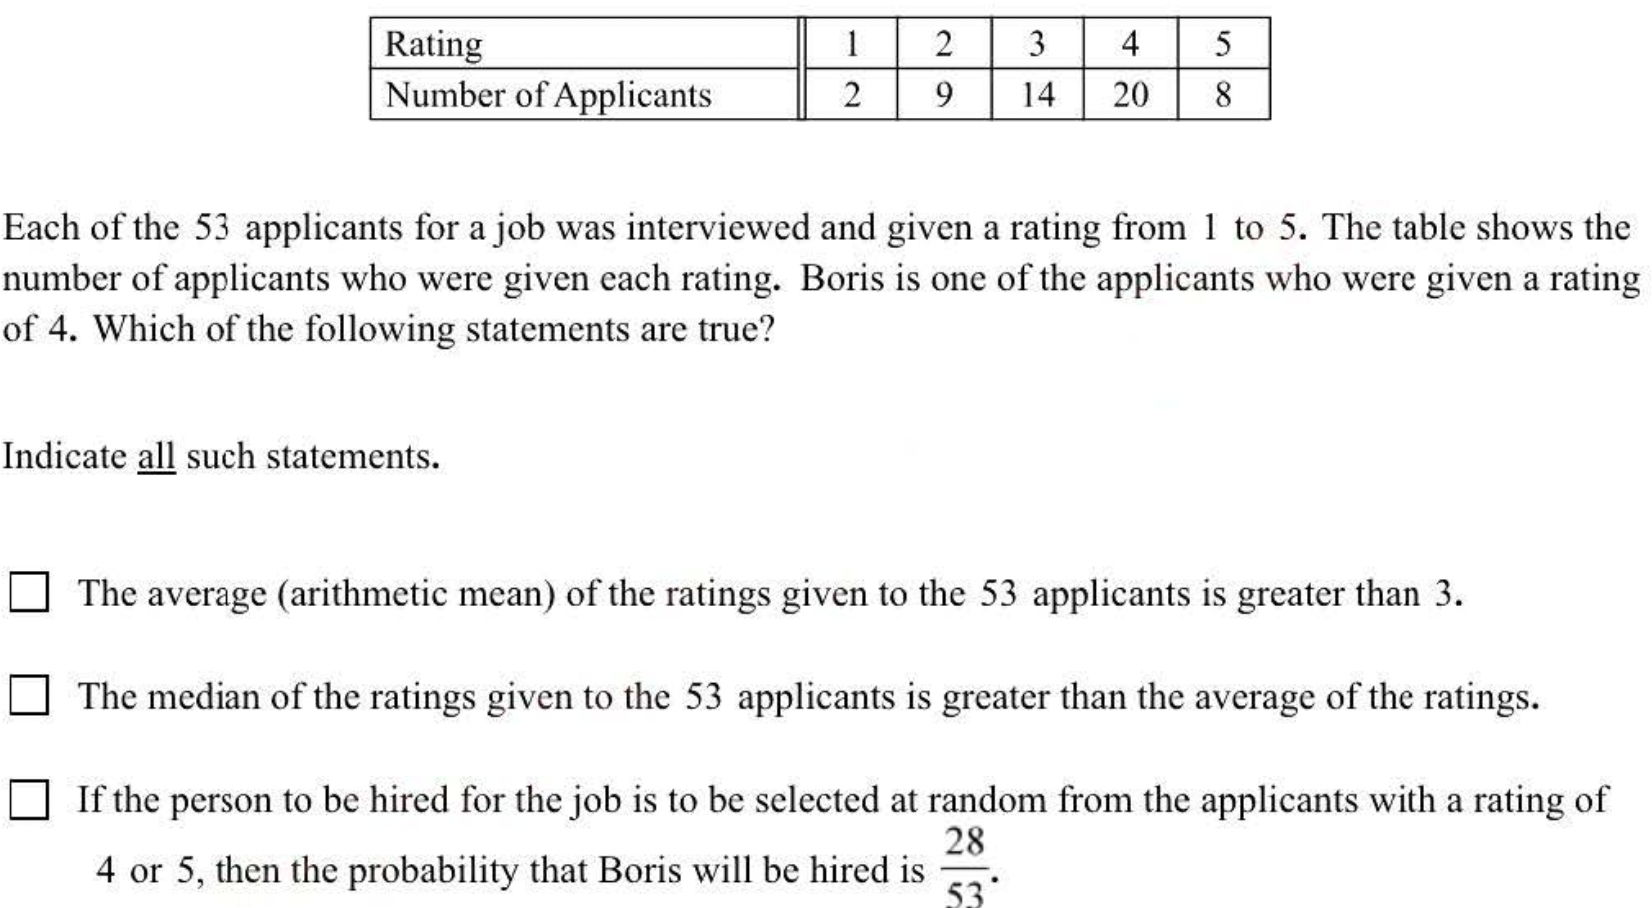
\includegraphics[width=\linewidth]{Conditional_Probability_Example_Question.png}
		\caption{6-Sec2-18}
	\end{figure}


\end{frame}

%------------------------------------------------

\begin{frame}
	\frametitle{Answer}
	\begin{itemize}
		\item	Average(Arithmetic Mean): $\bar{x} =3.43 $ > 3
		\item Median: $Q_2 = 4 > mean = 3.43$ 
		\item $P("Hire Boris" | "Hire someone with 4 or 5 rating randonly") = \frac{1}{28}$
	\end{itemize}
	\pause
	\bigskip
	Answer \textbf{AB } \alert{We have better ways to compare median and mean later!}
\end{frame}

%------------------------------------------------
\subsection{Independent Events}


%------------------------------------------------


\begin{frame}
	\frametitle{Independent Events}
	\framesubtitle{独立事件互不影响可以同时发生}
	
	\begin{definition}
	 $$P(A\mid B) = P(A)$$
	 $$P(A and B) = P(A) P(B)$$

	\end{definition}
	\begin{example}
		Event $H_1$: A coin tossed shows head.
		Event $H_2$: A another coin tossed shows head.\\
		$P(H_1 and H_2)  = P(H_1)P(H_2) =\frac{1}{2}\frac{1}{2} = \frac{1}{4}$
	\end{example}
\end{frame}

%------------------------------------------------

\begin{frame}
	\frametitle{Can Independents Events Be Mutually Exclusive? }
	\framesubtitle{独立不互斥,互斥不独立}
	\begin{theorem}
Note that if $P(E) \neq 0 $ and $P(F) \neq 0$, then events  and F cannot be
both mutually exclusive and independent.		
	\end{theorem}
	\pause
	\begin{proof}
		If E and F are mutually exclusive, $P(A|B) = 0 \neq P(A) $. Vice versa. 
	\end{proof}
\end{frame}

%------------------------------------------------

\begin{frame}
	\frametitle{A Real QR Problem!}
	\framesubtitle{}
	\begin{figure}
		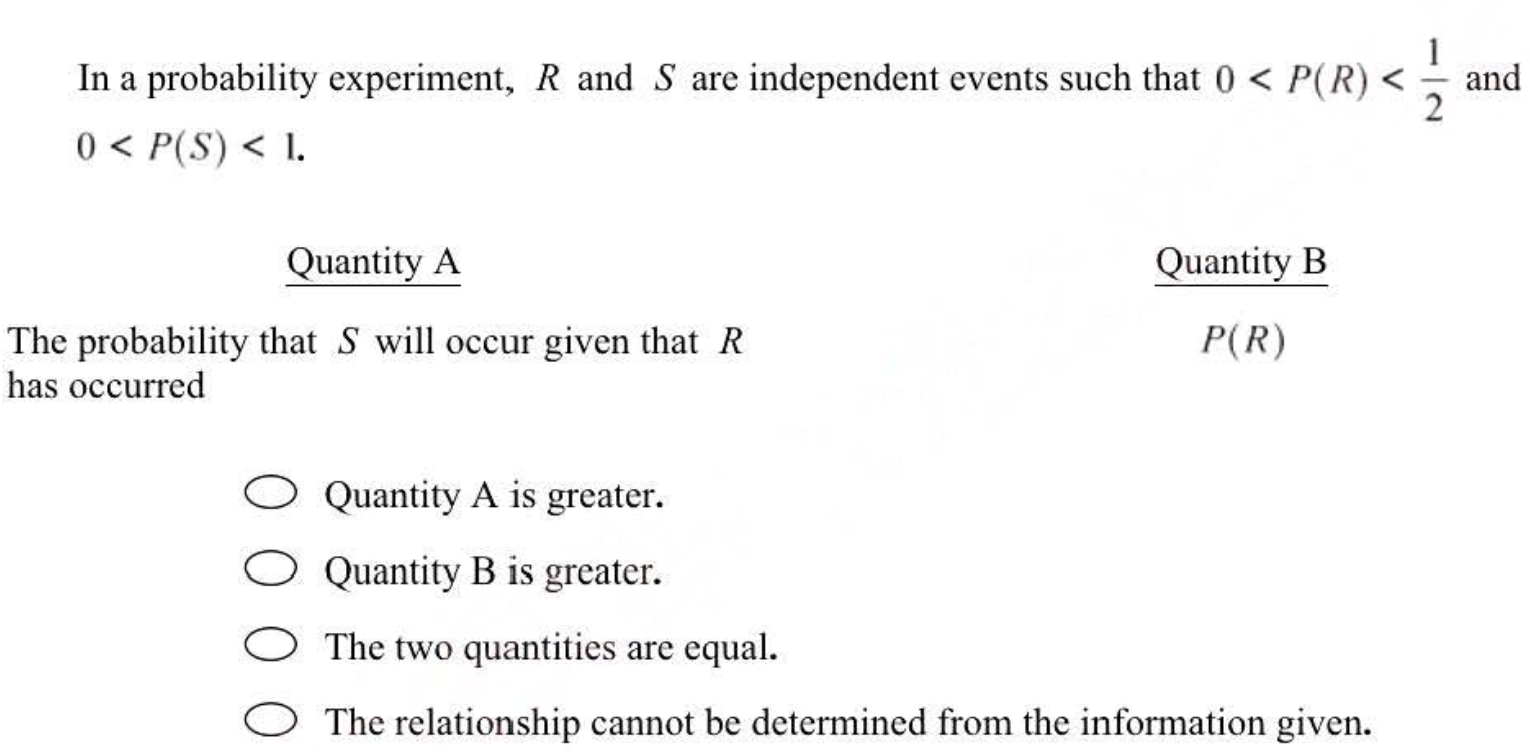
\includegraphics[width=0.8\linewidth]{Independent_Example_Question1.png}
		\caption{5-Sec3-6}
	\end{figure}
	\pause
$P(S\mid R) = P(S)$ \\
\pause
\bigskip
Answer \textbf{D} 
\end{frame}

%------------------------------------------------

\section{Descriptive Data Analysis (Exploratory Data Analysis)}

%------------------------------------------------



\subsection{Data Type}

%------------------------------------------------

\begin{frame}
	\frametitle{Quantitative V.s. Categorical }
	\framesubtitle{看能不能求平均}
	\begin{columns}[t] 
		\begin{column}{0.5\textwidth} % Left column width
		\textbf{Quantitative Variables}\\
		 \begin{definition}
		 	It make sense to calculate the mean of a quantitative variable.
		 \end{definition}
		 \begin{example}
		 	age, height, weight, GRE QR score
		 \end{example}
		\end{column}

		\begin{column}{0.5\textwidth} % Right column width
				\textbf{Categorical Variables}\\
		 \begin{definition}
		 	It doesn't make sense to calculate the mean of a categorical variable.
		 \end{definition}
		 \begin{example}
		  eye color, gender, district, native language
		 \end{example}
    \end{column}
	\end{columns}
\end{frame}



\subsection{Methods for Presenting Data}

%------------------------------------------------

\begin{frame}
	\frametitle{Distribution }
	\framesubtitle{变量的值如何分布}
	\begin{definition}
		The distribution of a variable, or distribution of data, indicates how
frequently different categorical or numerical data values are observed in the
data. Namely, a distribution shows
\begin{itemize}
	\item the values of the variables
	\item the frequencies of those values
\end{itemize}
	\end{definition}
\end{frame}

%------------------------------------------------
\begin{frame}
	\frametitle{Frequency Table}
	\framesubtitle{频率表} % Optional subtitle
	A survey was taken to find the number of children in each
of 25 families. A list of the 25 values collected in the survey follows.\\
1 2 0 4 1 3 3 1 2 0 4 5 2 3 2 3 2 4 1 2 3 0 2 3 1
	\begin{table}
		\begin{tabular}{l l }
			\toprule
			\textbf{Number of Children} & \textbf{Frequency}\\
			\midrule
			0 & 3 \\
			1 & 5 \\
			2 & 7 \\
			3 & 6 \\
			4 & 3 \\
			5 & 1 \\
			Total & 25\\
			\bottomrule
		\end{tabular}
		\caption{Frequency Distribution Of The Number Of Children}
	\end{table}
	\alert{Quantitative or Categorical}
\end{frame}

%------------------------------------------------

\begin{frame}
	\frametitle{Pie Charts}
	\framesubtitle{饼状图} % Optional subtitle

	\begin{figure}
		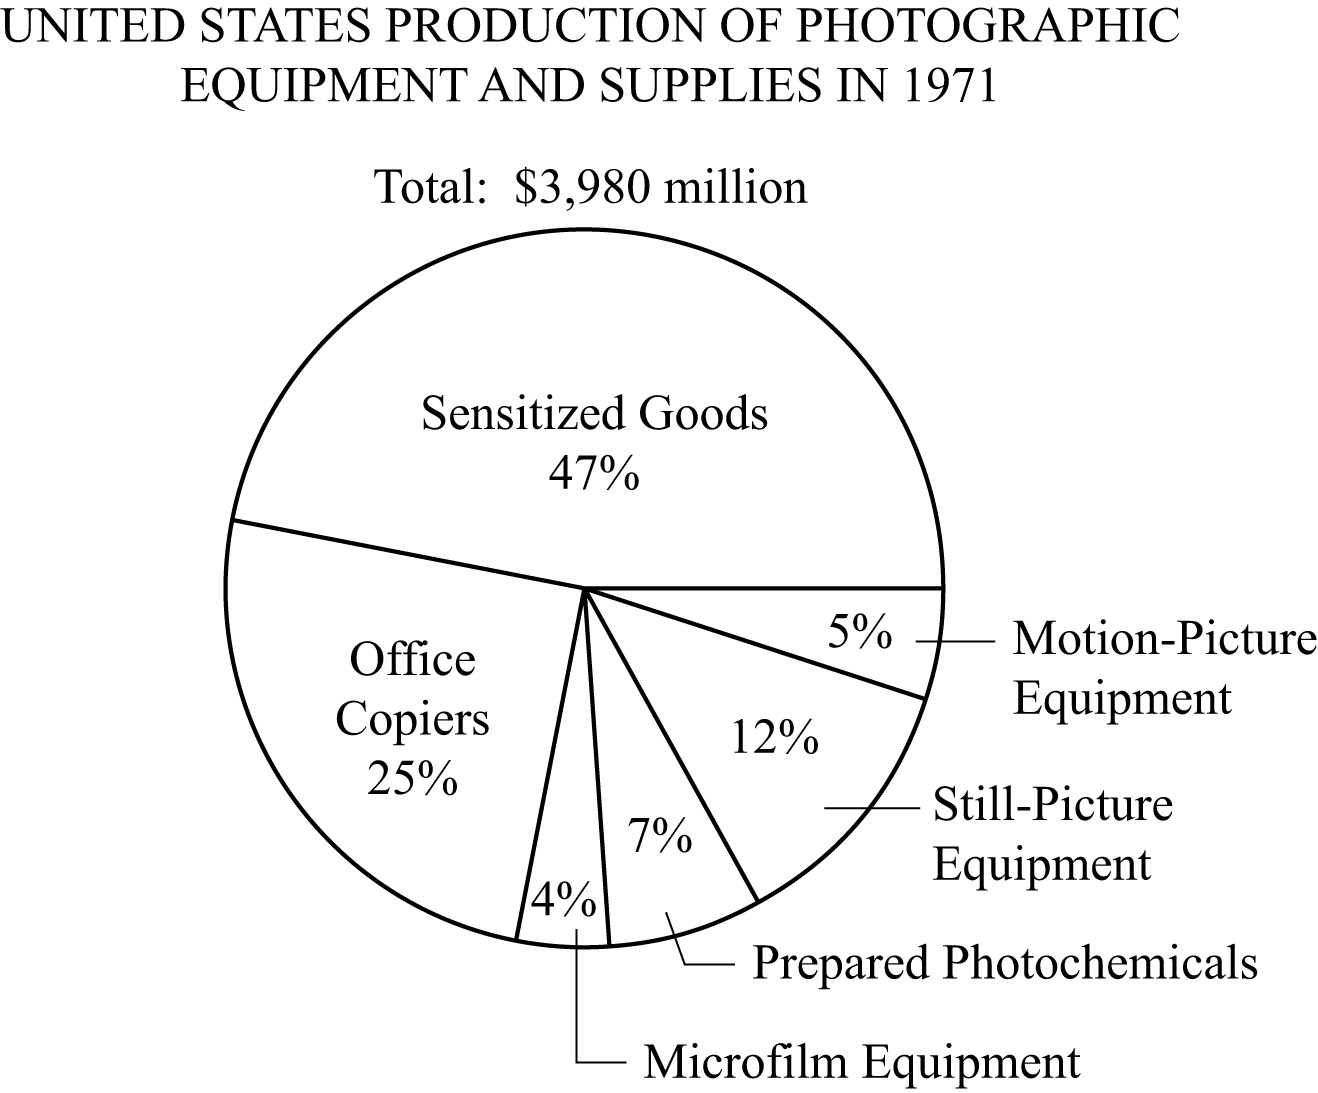
\includegraphics[width=0.5\linewidth]{Pie_Charts.jpg}
		\caption{6 sectors.}
	\end{figure}
	\alert{Categorical}
\end{frame}

%------------------------------------------------

\begin{frame}
	\frametitle{Bar Graph}
	\framesubtitle{柱状图} % Optional subtitle

	\begin{figure}
		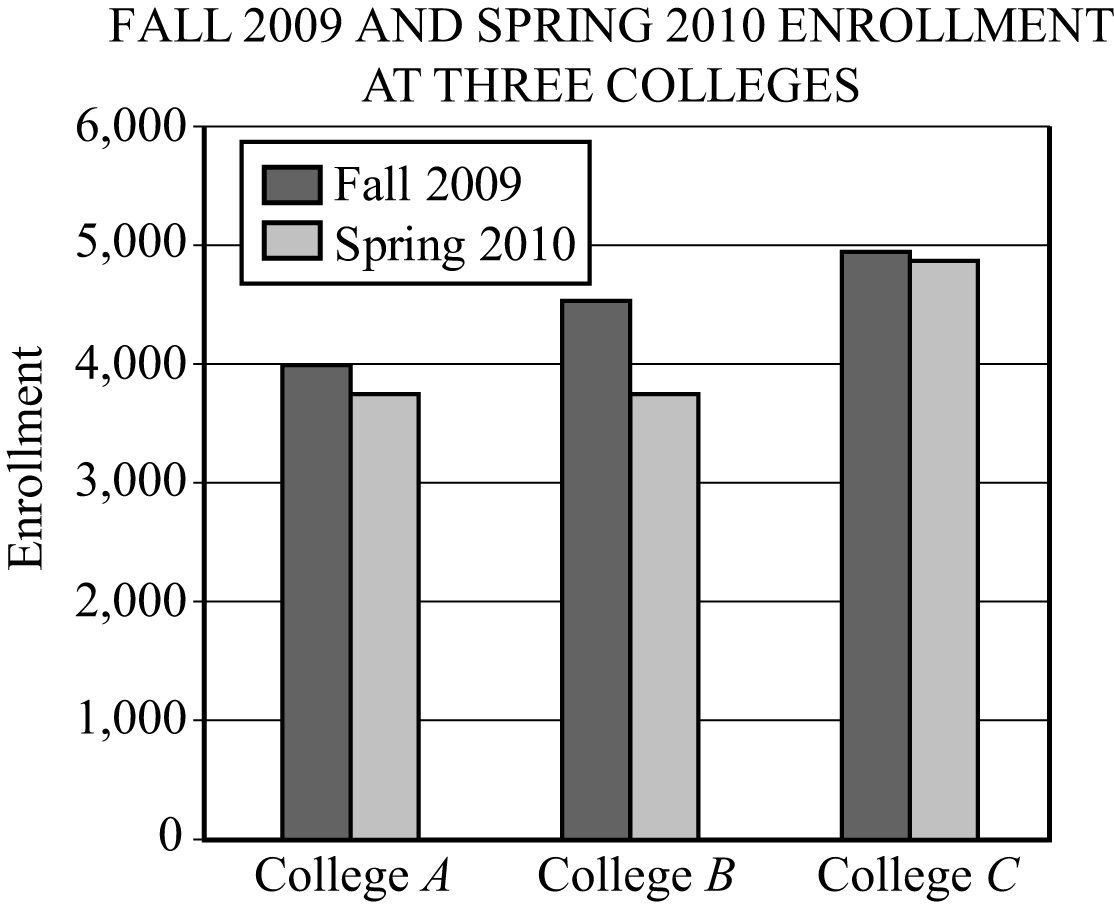
\includegraphics[width=0.5\linewidth]{Bar_Graph.jpg}
	\end{figure}
	\alert{Categorical Or Discrete Quantitative}
\end{frame}

%------------------------------------------------

\begin{frame}
	\frametitle{Segmented Bar Graph}
	\framesubtitle{堆叠柱状图} % Optional subtitle

	\begin{figure}
		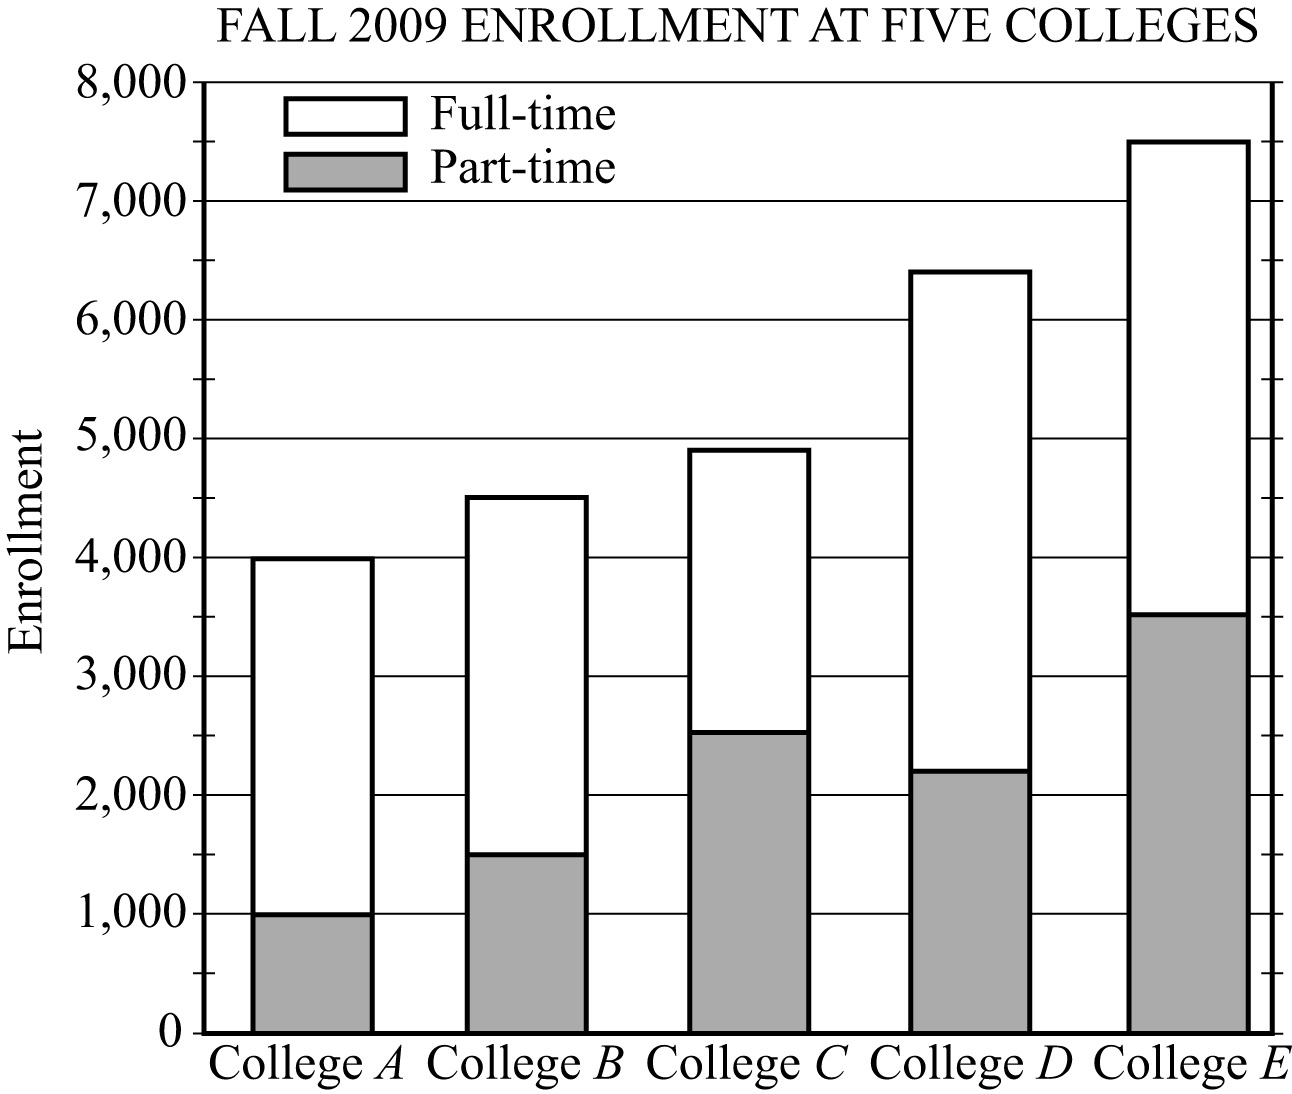
\includegraphics[width=0.5\linewidth]{Segmented_Bar_Graph.jpg}
	\end{figure}
	\alert{Categorical-Categorical}
\end{frame}

%------------------------------------------------

\begin{frame}
	\frametitle{Histogram}
	\framesubtitle{条形图} % Optional subtitle

	\begin{figure}
		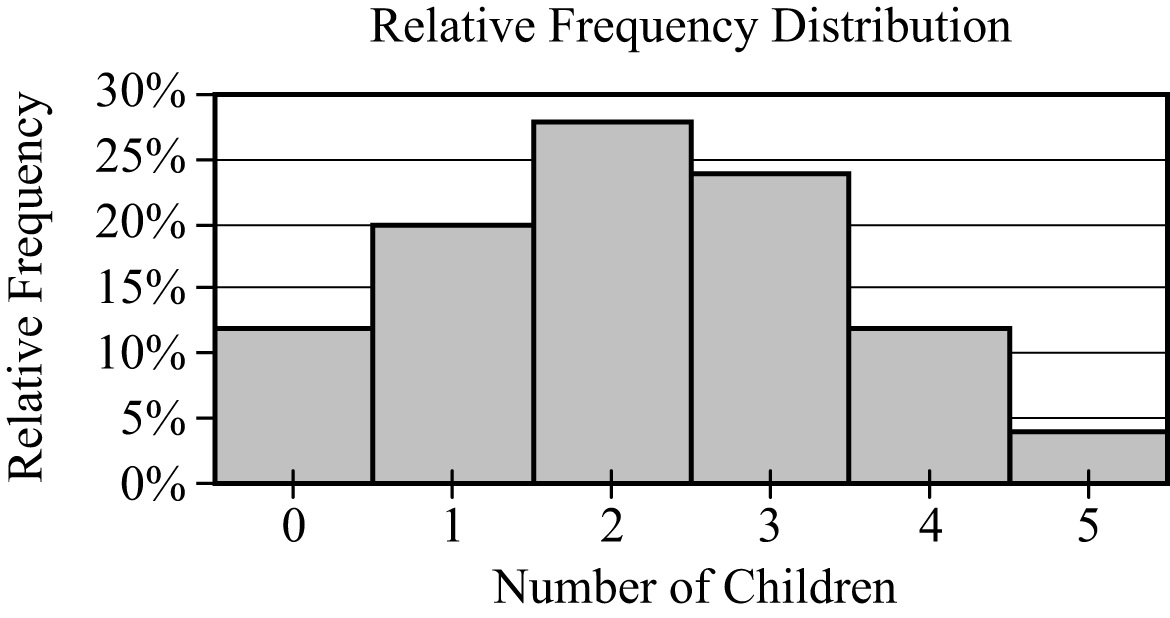
\includegraphics[width=0.5\linewidth]{Histogram.jpg}
	\end{figure}
	\alert{Continuous Quantitative}
\end{frame}

%------------------------------------------------

\begin{frame}
	\frametitle{Line Graph}
	\framesubtitle{折线图} % Optional subtitle

	\begin{figure}
		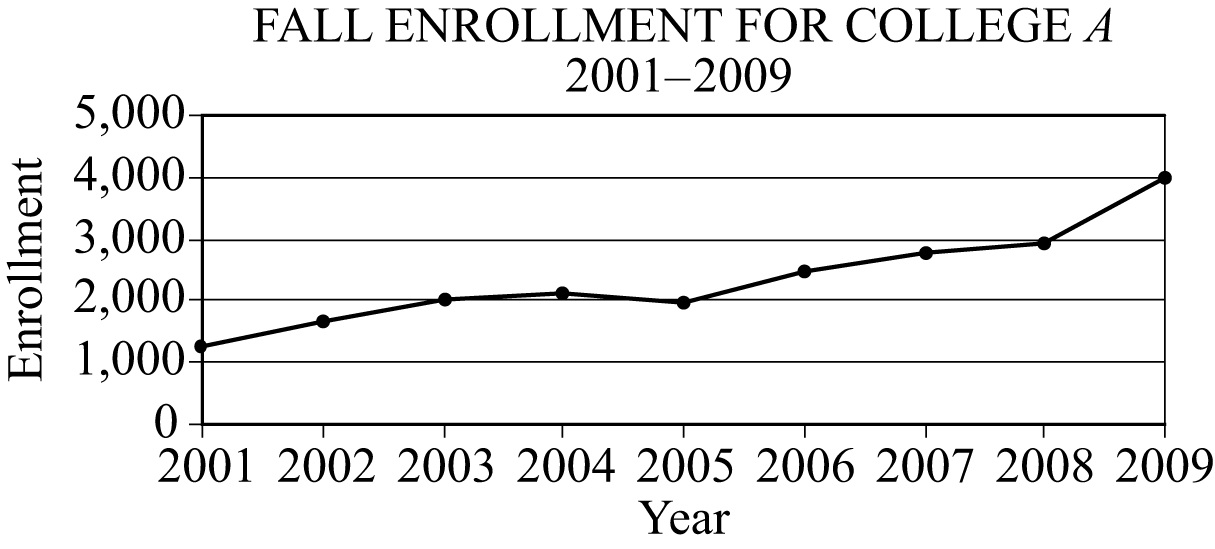
\includegraphics[width=0.5\linewidth]{Line_Graph.jpg}
	\end{figure}
	\alert{Quantitative in time series}
\end{frame}

%------------------------------------------------


\begin{frame}
	\frametitle{Scatter plot}
	\framesubtitle{散点图} % Optional subtitle

	\begin{figure}
		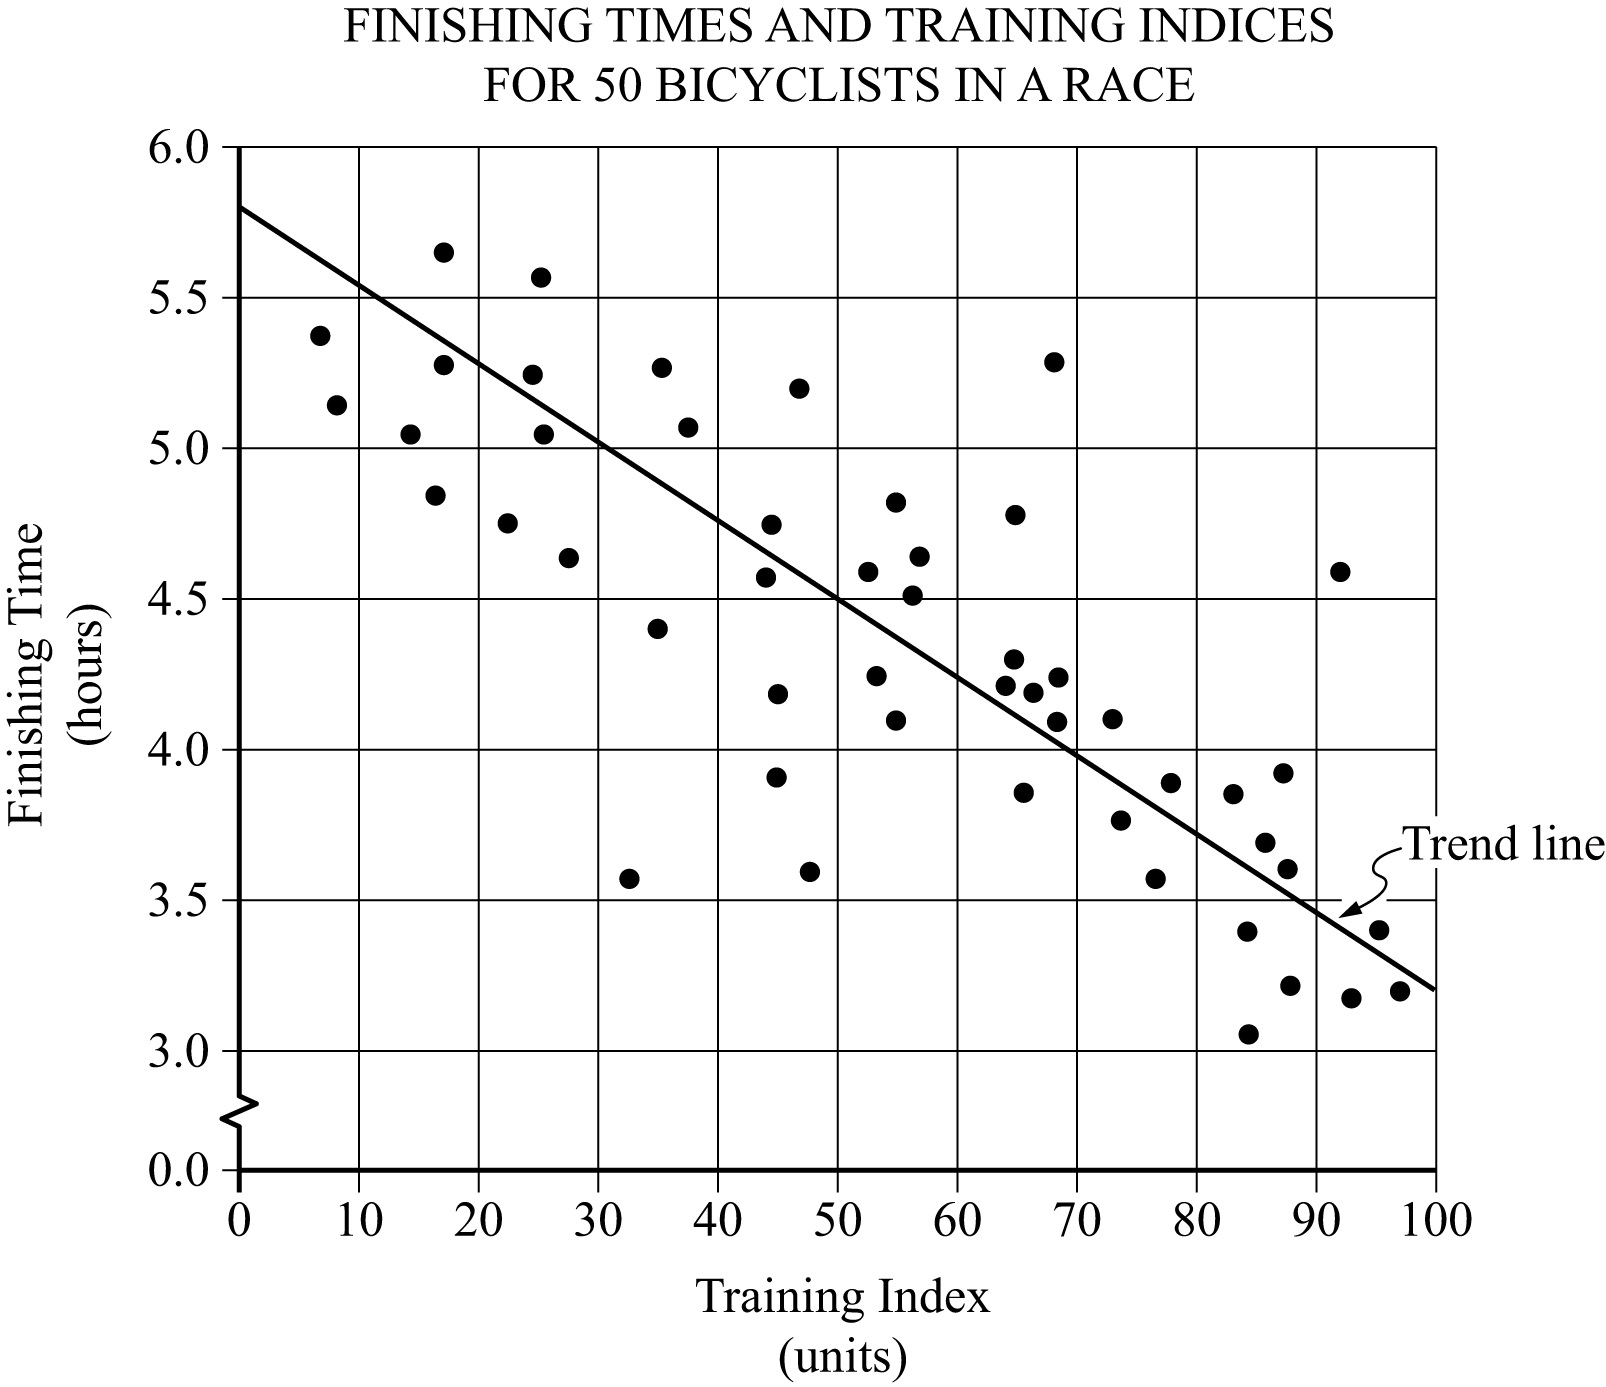
\includegraphics[width=0.5\linewidth]{Scatter_Plot.jpg}
	\end{figure}
	\alert{Quantitative-Quantitative}\\
	The slope can be interpreted as follows: The finishing time is \alert{predicted}to
decrease 0.026 hour for every unit by which the training index increases.\\
\alert{The regression line is not observed data but a theoretical model.}
\end{frame}

%------------------------------------------------

\begin{frame}
	\frametitle{Nota Bene} % Slide title, remove this command for no title
	\framesubtitle{重点!}

	\begin{block}{QR Mathematical Convention 5}
		When graphical data presentations, such as bar graphs and line graphs,
are shown with scales, you should read, estimate, or compare quantities
by sight or by measurement, according to the corresponding scales.
	\end{block}

		\begin{block}{QR Mathematical Convention 4}
		Scales, grid lines, dots, bars, shadings, solid and dashed lines, legends,
etc., are used on graphs to indicate the data. Sometimes scales that do not
begin at 0 are used, and sometimes broken scales are used..
	\end{block}
	\begin{alertblock}{看图要点}
		\begin{itemize}
			\item Carefully understand title, the labels for x-axis and y-axis, and legends.看标题,XY轴,图例找到数据的含义
			\item Carefully examine the scales and unit.看单位
			\item Carefully examine the the starting point.看起点
		\end{itemize}
	\end{alertblock}
\end{frame}

%------------------------------------------------

\begin{frame}
	\frametitle{How to read a graph} % Slide title, remove this command for no title
	\framesubtitle{读图要点}
	\begin{figure}
		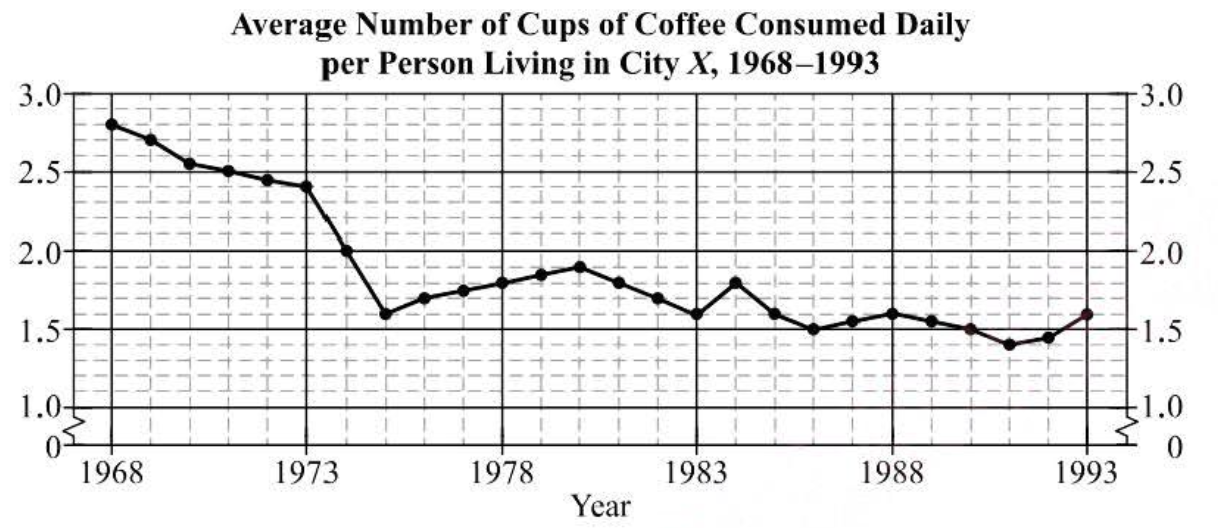
\includegraphics[width=0.8\linewidth]{Graph.png}
		\caption{The graph shows The trends of The average number of cups of coffee consumed daily
per person living in city X by year. Y suggest number of cups. X suggest the year. Y use a broken scales.}
	\end{figure}
\end{frame}

%------------------------------------------------

\subsection{Measures of Central Tendency}

%------------------------------------------------

\begin{frame}
	\frametitle{Mode}
	\framesubtitle{众数}
	\begin{definition}
		The mode of a list of numbers is the number that occurs most frequently
in the list.
	\end{definition}
	\begin{example}
		1, 2, 3, 3, 3, 5, 7, 10, 10, 10, 20 has two modes, 3 and 10.
	\end{example}
	\alert{There could be more than one mode.}
\end{frame}

%------------------------------------------------

\begin{frame}
	\frametitle{Median}
	\framesubtitle{中值}
	\begin{definition}
	The median is the middle number in a sorted, ascending or descending, list of numbers.
	\end{definition}
	\begin{example}
		1, 2, 3, 3, 3, 5, 7, 10, 10, 10, 20 has a median 5.
		1, 2, 3, 3, 3, 5, 7, 10, 10, 10 has a median $\frac{3 + 5}{2} = 4$.
	\end{example}
\end{frame}

%------------------------------------------------

\begin{frame}
	\frametitle{Mean}
	\framesubtitle{平均数}
	\begin{definition}
	$$\bar{x} =  \sum freq(x) \cdot x$$
	\end{definition}
	\begin{example}
		2, 4, 4, 5, 7, 7, 7, 7, 7, 7, 8, 8, 9, 9, 9, 9\\
		$$mean = \frac{1(2) + 2(4) +  1(5) + 6(7) + 2(8) + 4(9)}{1 + 1 + 6 + 2 + 4} = 6.8125$$
	\end{example}
\end{frame}

%------------------------------------------------

\begin{frame}
	\frametitle{Mean v.s. Median}
	\framesubtitle{平均数 V.s. Median}

	{\LARGE Which one of median and mean are more influenced by extreme values?}
	\pause
	\bigskip\bigskip\bigskip\bigskip
	Answer \textbf{Mean}
\end{frame}

%------------------------------------------------

\begin{frame}
	\frametitle{Skewness}
	\framesubtitle{“斜”就是extreme values}
	\begin{figure}
		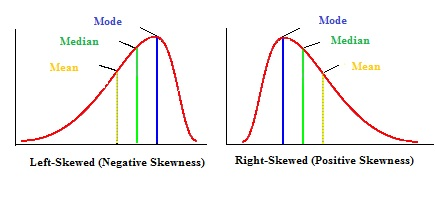
\includegraphics[width=0.8\linewidth]{Skewness.jpeg}
	\end{figure}
\end{frame}

%------------------------------------------------
\begin{frame}
	\frametitle{Is QR Score Right-Skewed or Left-Skewed?}
	\framesubtitle{左斜还是右斜?}

	\bigskip % Vertical whitespace
	\begin{table}
		\begin{tabular}{l l l l}
			\toprule
			\textbf{GRE Quantitative Score} & \textbf{2019} & \textbf{2020} & \textbf{2021}\\
			\midrule
			Mean & 169.1 & 169.5 & 169.17 \\
			Median & 160.0 & 160.7 & 161.9 \\
			\bottomrule
		\end{tabular}
		\caption{The median and average GRE QR score for the entering class of 2019, 2020 and 2021 in Mathematics of Finance MA Program of Columbia University}
	\end{table}

	\pause
	Answer \textbf{Right-Skewed} \alert{What if mean equals median?}
\end{frame}

%------------------------------------------------

\begin{frame}
	\frametitle{A Real QR Problem!}
	\framesubtitle{}
	\begin{figure}
		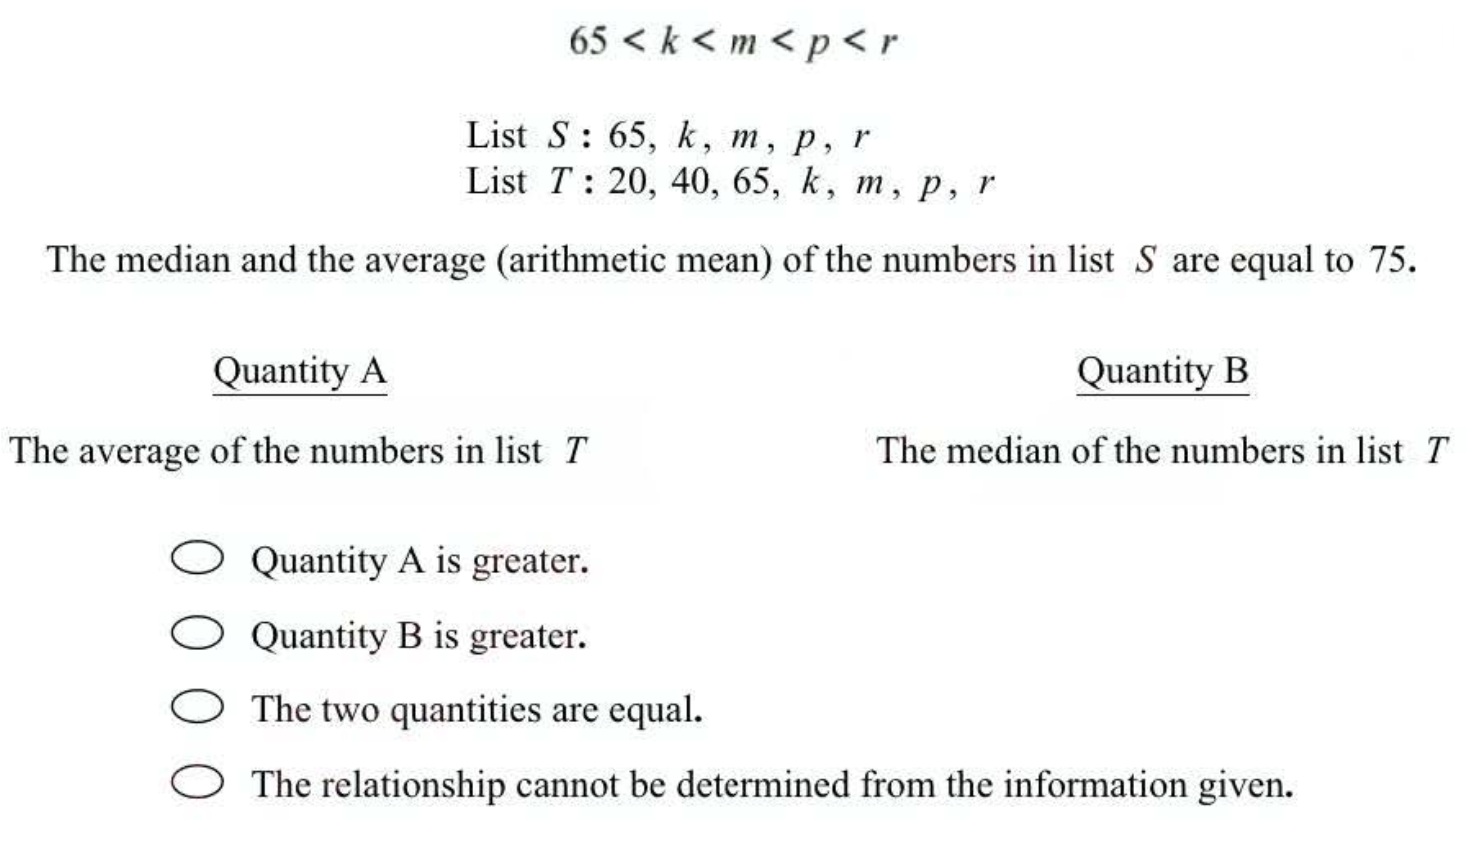
\includegraphics[width=\linewidth]{Median.png}
		\caption{7-Sec2-1}
	\end{figure}

\end{frame}

%------------------------------------------------

\begin{frame}
	\frametitle{A Real QR Problem!}
	\framesubtitle{}
	\begin{figure}
		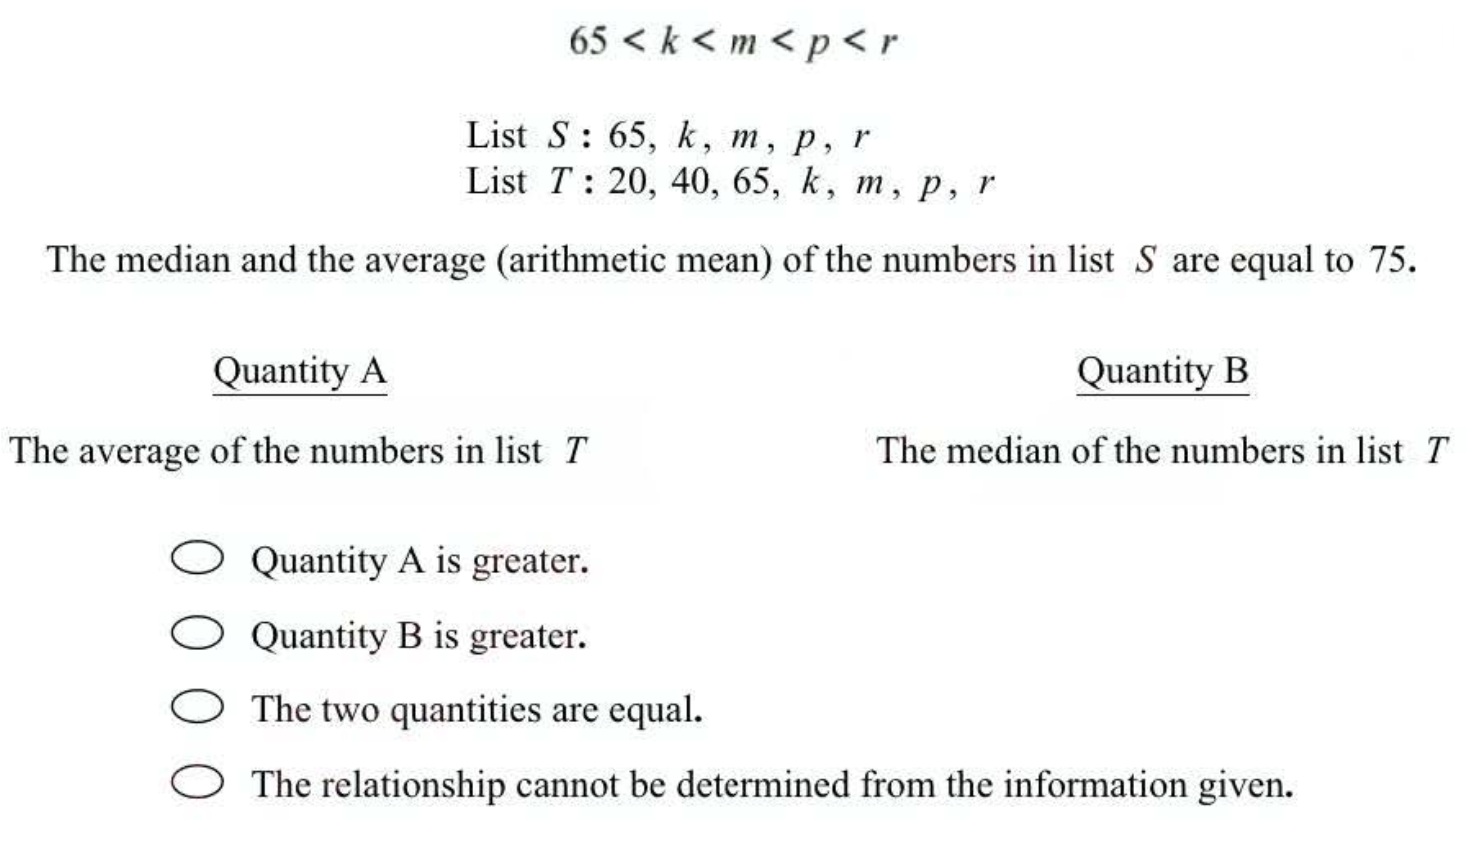
\includegraphics[width=\linewidth]{Median.png}
		\caption{7-Sec2-1}
	\end{figure}
	\pause
 \pause
\bigskip
Answer \textbf{B } 
\end{frame}

%------------------------------------------------


\subsection{Measures of Position}

%------------------------------------------------

\begin{frame}
	\frametitle{Quartile}
	\framesubtitle{三个四等分点}
	\begin{definition}
	There are three
quartile numbers, called the first quartile $Q_1$, the second quartile $Q_2$, and the third
quartile $Q_3$, that divide the data into four roughly equal groups.
	\end{definition}
	\begin{example}
	16 numbers: 2, 4, 4, 5, 7,7, 7, 7, 7, 7, 8, 8, 9, 9, 9, 9\\
	\begin{enumerate}
		\item Divide the list into  the 2 group of 8 numbers
		\item Group 1:\quad   2, 4, 4, 5, 7,7, 7, 7;   Group 2:\quad  7, 7, 8, 8, 9, 9, 9, 9.
		\item The average of the last number of group 1 and the first number of group 2 is $Q_2=\frac{7+7}{2}=7$.
		\item similarly, The median of the group 1 is $Q_1=\frac{5+7}{2}=6$
		\item similarly, The median of the group 2 is $Q_3=\frac{8+9}{2}=8.5$
	\end{enumerate}
		\alert{偶数个数要把median算入分别算入the first half and the second half}

	\end{example}
\end{frame}

%------------------------------------------------

\begin{frame}
	\frametitle{Quartile For a List with Odd-number Elements}
	\framesubtitle{奇数个数不包含median 分成两半}

	\begin{example}
	11 Numbers: 6, 7, 15, 36, 39, 40, 41, 42, 43, 47, 49\\
	\begin{enumerate}
		\item The 6th element is $Q_2=40$.
		\item Divide the list into  the 2 group of 5 numbers, excluding the $Q_2$
		\item Group 1:\quad   6, 7, 15, 36, 39;   Group 2:\quad  41, 42, 43, 47, 49.
		\item similarly, The median of the group 1 is $Q_1=15$
		\item similarly, The median of the group 2 is $Q_3=43$
	\end{enumerate}
	\end{example}
\end{frame}

%------------------------------------------------

\begin{frame}
	\frametitle{Percentile}
	\framesubtitle{99个点等分100份}
	\begin{definition}
	there are 99
percentile numbers that divide the data into 100 roughly equal groups.
	\end{definition}

\end{frame}

%------------------------------------------------


\begin{frame}
	\frametitle{Standardized Score}
	\framesubtitle{Z-Score}
	\begin{definition}
	\begin{equation*}
		z = \frac{x - \mu}{\sigma}
	\end{equation*}
	\end{definition}
	\alert{距离平均值的center有几个$\sigma$远}
\end{frame}

%------------------------------------------------

\subsection{Measures of Dispersion}

%------------------------------------------------

\begin{frame}
	\frametitle{Dispersion}
	\framesubtitle{数据的离散程度}
	{\LARGE 下面那个分布更加团结?数据直接更相同?} y轴表示frequency.
		\begin{figure}
		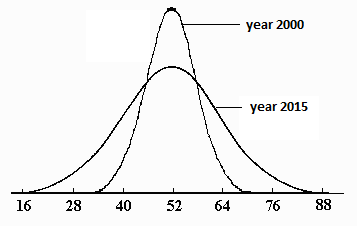
\includegraphics[width=0.7\linewidth]{Dispersion.png}
	\end{figure}
\end{frame}

%------------------------------------------------


\begin{frame}
	\frametitle{Range}
	\framesubtitle{极差}
	\begin{definition}
		\begin{equation*}
			Range = Maxium - Minimum
		\end{equation*}
	\end{definition}
	\pause
	\alert{Are Range influenced by outliers?} \pause Yes!
\end{frame}

%------------------------------------------------


\begin{frame}
	\frametitle{Interquartile Range}
	\framesubtitle{IQR: quartile之间的range}
	\begin{definition}
		\begin{equation*}
			IQR = Q_3 - Q_1
		\end{equation*}
	\end{definition}
\begin{example}
In the list of 16 numbers 2, 4, 4, 5, 7, 7, 7, 7, 7, 7, 8, 8, 9, 9,
9, 9, the range is 9 − 2 = 7, the first quartile,$Q_1 = 6$ , and the third quartile, $Q_3 = 8.5$. So the interquartile range for the numbers in this list is $8.5 - 6 = 2.5$.
		\begin{figure}
		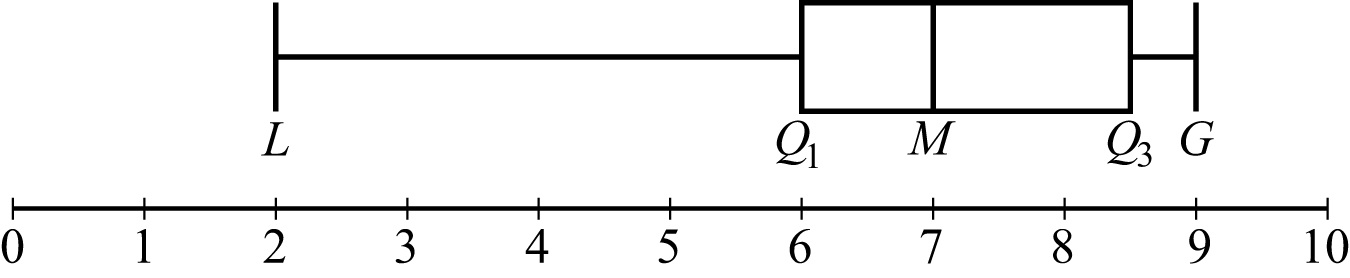
\includegraphics[width=0.7\linewidth]{IQR.jpg}
	\end{figure}
\end{example}
	\pause
	\alert{Are IQR influenced by outliers?} \pause No!
\end{frame}

%------------------------------------------------

\begin{frame}
	\frametitle{Standard Deviation}
	\framesubtitle{标准差}
	\begin{definition}
	Population Standard Deviation:
		\begin{equation*}
			\sigma = \sqrt{\frac{\sum (x - \mu)^2}{n}}
		\end{equation*}
			Sample Standard Deviation:
		\begin{equation*}
			S_x = \sqrt{\frac{\sum (x - \mu)^2}{n-1}}
		\end{equation*}
	\end{definition}
	\pause
	\alert{Are std influenced by outliers?} \pause Yes!
\end{frame}

\subsection{Linear Transformation of Datasets}
%------------------------------------------------
% TO-DO: Linear Transformation

\begin{frame}
	\frametitle{Linear Transformation of Datasets}
	\framesubtitle{数据集的线性变换}
	\begin{theorem}
		Let $X = {x_1, x_2, \cdots x_n}$ and $Y = aX + b$. Then,
		$\mu_y = a\mu_x + b \quad \quad \quad\sigma_y = a\sigma_x$
	\end{theorem}
	\begin{columns}[t] 
		\begin{column}{0.45\textwidth} % Left column width
		\begin{proof}
		\begin{equation*}
			\begin{aligned}
				\mu_y &= \frac{\sum y}{n}\\
				      &= \frac{\sum ax + b}{n}\\
				      &= a \frac{\sum x}{n} + b\\
				      &= a \mu_x + b
			\end{aligned}
		\end{equation*}
		\end{proof}

		\end{column}
		\begin{column}{0.5\textwidth} % Right column width
				\begin{proof}
				\begin{equation*}
					\begin{aligned}
						Range_y = a Range_x  &= \sqrt{\frac{\sum [(ax + b) - (a\mu_x + b)]^2}{n}}\\
						         &= a\sqrt{\frac{\sum (x  - \mu_x )^2}{n}}= a \sigma_x
					\end{aligned}
				\end{equation*}
				\end{proof}
		\end{column}
	\end{columns}
\end{frame}

%------------------------------------------------


\begin{frame}
	\frametitle{Linear Transformation of Datasets}
	\framesubtitle{数据集的线性变换}
	\begin{columns}[t] 
		\begin{column}{0.45\textwidth} % Left column width
		\begin{definition}
			a scales the data distribution and will influence the dispersion as well as the central tendency.
		\end{definition}
		\end{column}
		\begin{column}{0.5\textwidth} % Right column width
		b shifts the data distribution and will not influence the dispersion.
		\end{column}
	\end{columns}
\end{frame}

%------------------------------------------------

\begin{frame}
	\frametitle{Linear Transformation of Datasets}
	\framesubtitle{数据集的线性变换}
	{\LARGE what about range, IQR, $Q_2$, and mode?}
	\pause
	\begin{theorem}
		Let $X = {x_1, x_2, \cdots x_n}$ and $Y = aX + b$. Then,
		$$Range_y = a \cdot Range_x$$ 
		$$IQR_y = a \cdot IQR_x$$
		$$Q_{2y} = a\cdot Q_{2x} + b$$
		$$mode_y = a\cdot mode_x + b $$
	\end{theorem}
\end{frame}


%------------------------------------------------

\section{Random Variables and Probability Distribution}

%------------------------------------------------

\subsection{Random Variables and Probability Distribution}

%------------------------------------------------

\begin{frame}
	\frametitle{Density Curve}
	\framesubtitle{概率密度函数}
	\begin{figure}
		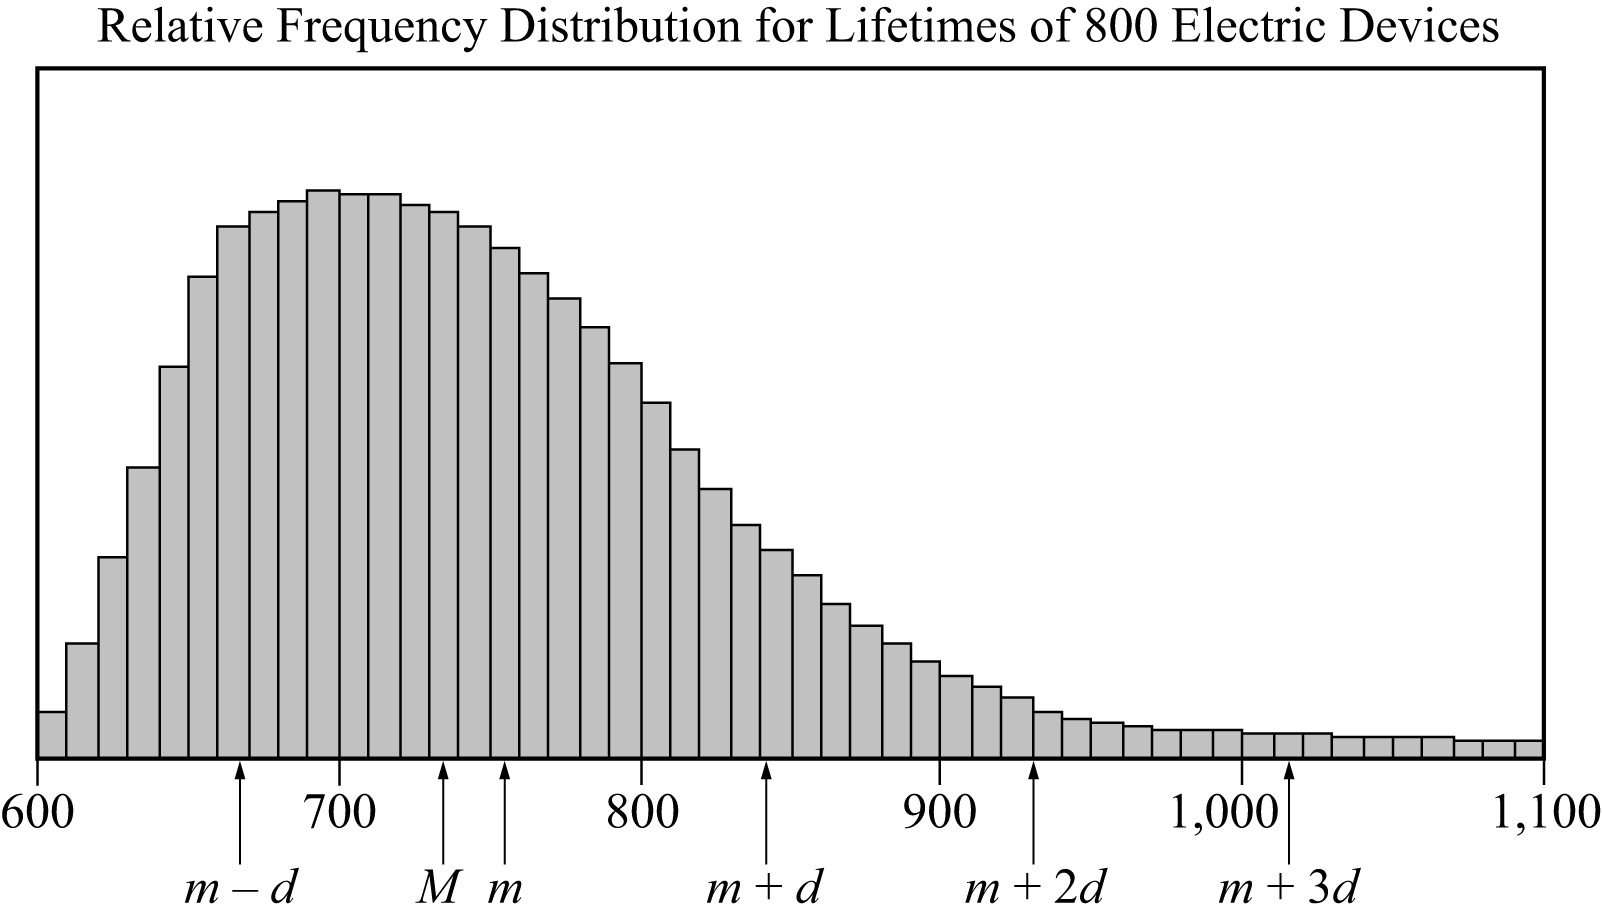
\includegraphics[width=0.8\linewidth]{Density_Curve.jpg}
		\caption{The area enclosed by the curve and x-axis is 1.}
	\end{figure}
\end{frame}

%------------------------------------------------


\begin{frame}
	\frametitle{Random Variables}
	\framesubtitle{随机变量}
	\begin{definition}
		a quantity having a numerical value for each member of a group, especially one whose values occur according to a frequency distribution.
	\end{definition}
	\begin{example}
		\begin{itemize}
			\item the age of the person randomly selected from the Chinese population
			\item the gender of the person randomly selected from the Chinese  population
		\end{itemize}
	\end{example}
\end{frame}

%------------------------------------------------

\begin{frame}
	\frametitle{Expectation}
	\framesubtitle{随机变量}
	\begin{definition}
		\begin{equation*}
			E(x) = \sum x P(x)
		\end{equation*}
	\end{definition}
\end{frame}

%------------------------------------------------

\subsection{Normal Distribution}

%------------------------------------------------
\begin{frame}
	\frametitle{Density Curve}
	\framesubtitle{概率密度函数}
	\begin{figure}
		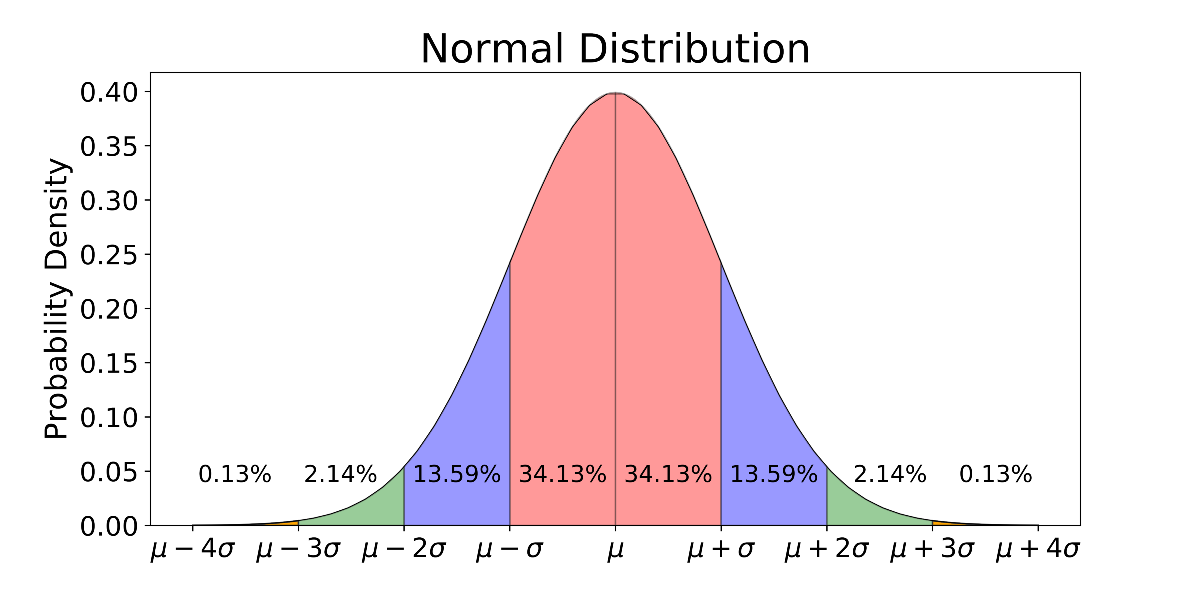
\includegraphics[width=0.8\linewidth]{Normal.png}
		\caption{The area in $\mu \pm \sigma$ is 68.27\%; The area in $\mu \pm 2\sigma$ is 95.45\%;  The area in $\mu \pm 3\sigma$ is 99.73\%.}
	\end{figure}
\end{frame}

%------------------------------------------------

\begin{frame}
	\frametitle{A Real QR Problem!}
	\framesubtitle{}
	\begin{figure}
		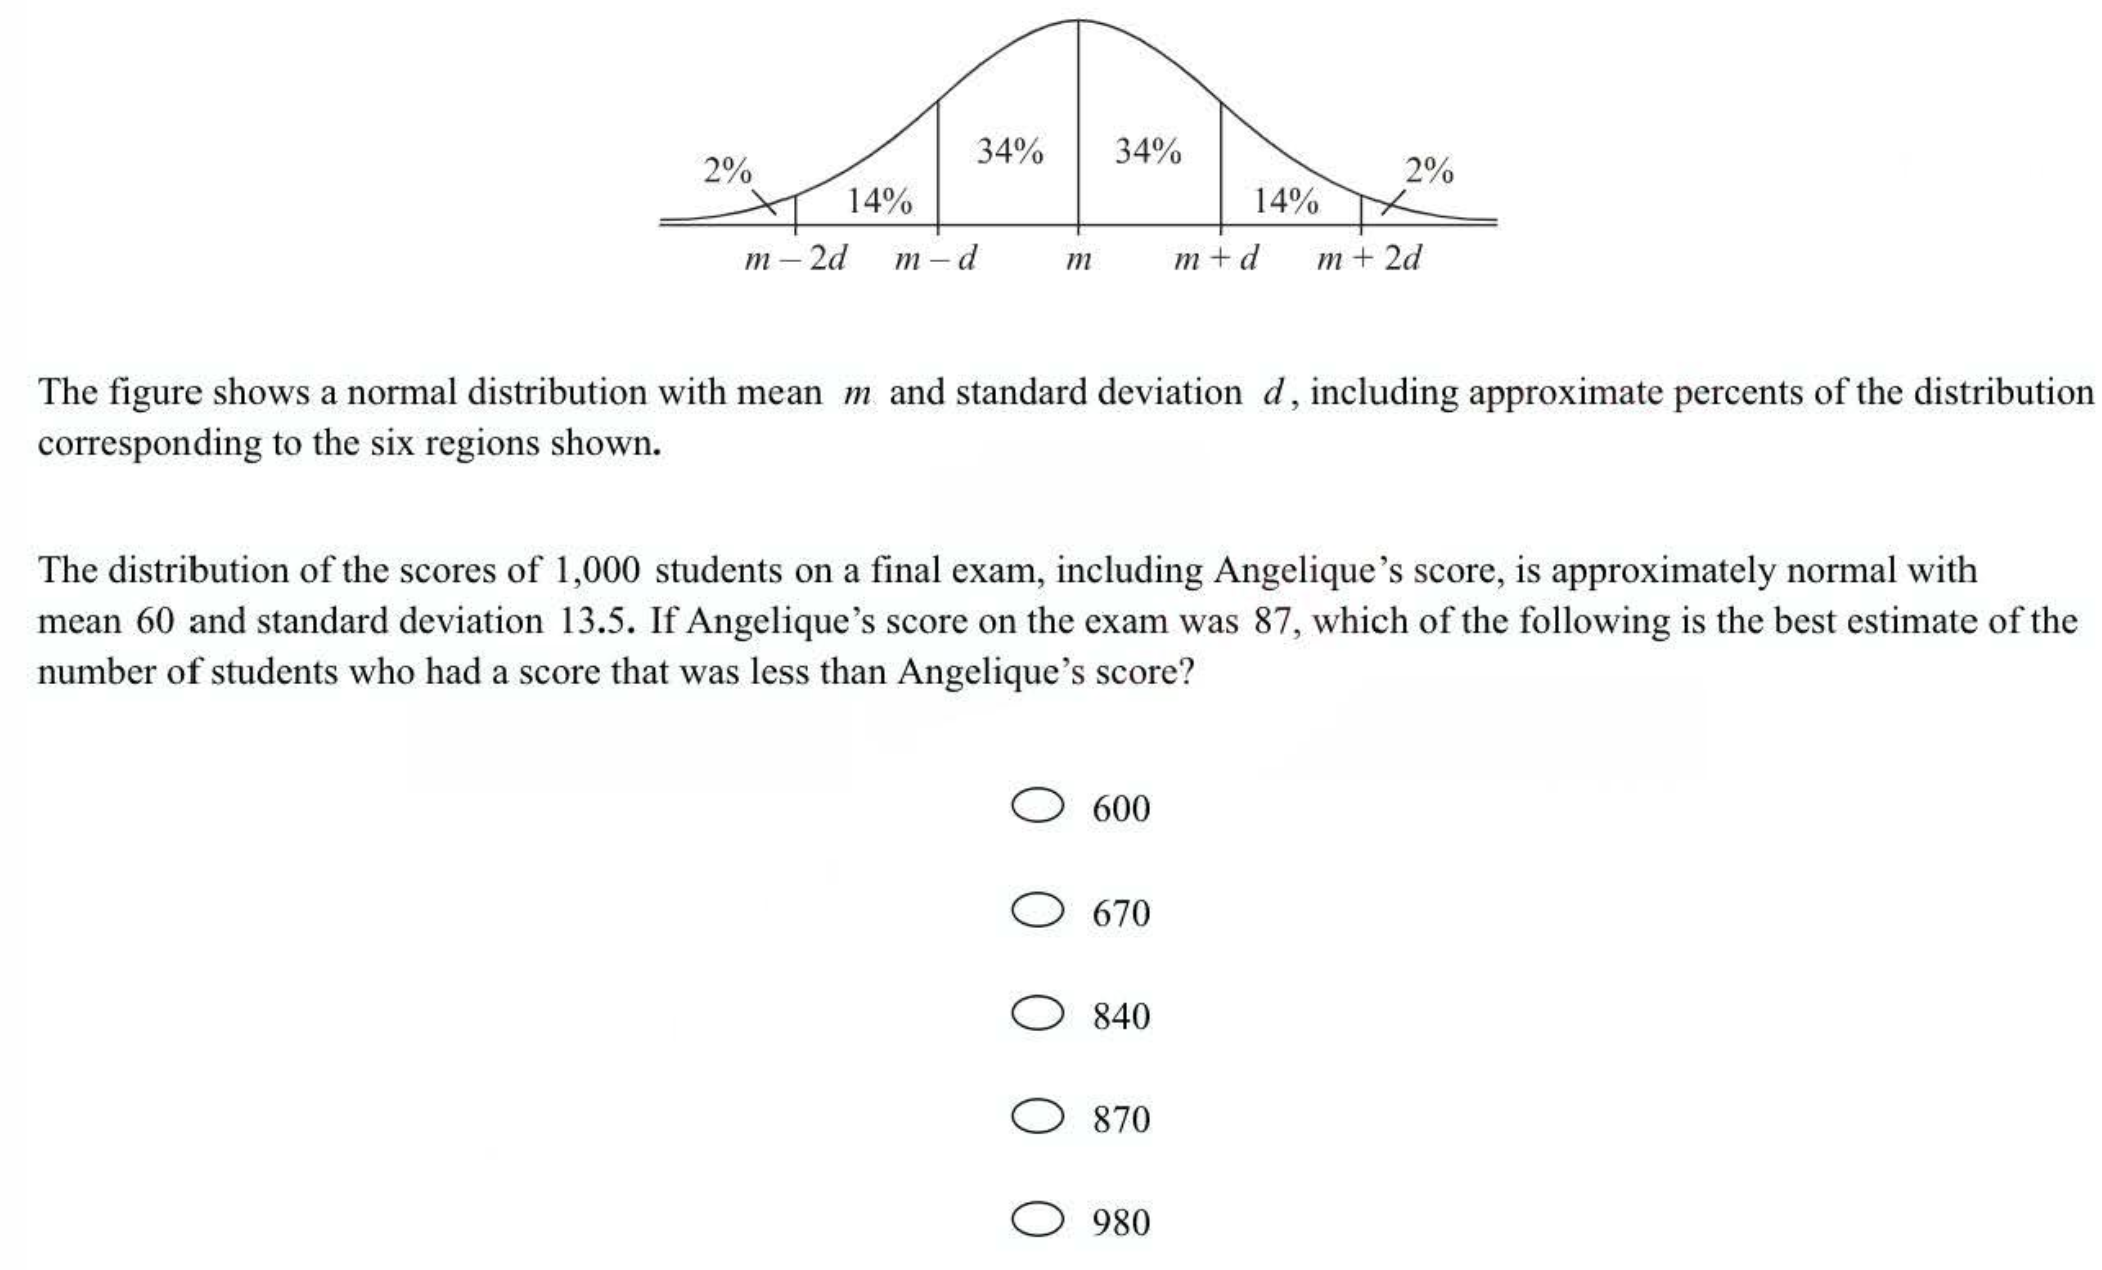
\includegraphics[width=\linewidth]{Normal_Example_Question.png}
		\caption{2-Sec2-9}
	\end{figure}
	\pause
$\frac{87 - 60}{13.5} = 2$\\
$1000 \times 98\% = 980$
\pause
\bigskip
Answer \textbf{E} 
\end{frame}

%------------------------------------------------



%----------------------------------------------------------------------------------------
%	CLOSING SLIDE
%----------------------------------------------------------------------------------------

\begin{frame}[plain] % The optional argument 'plain' hides the headline and footline
	\begin{center}
		{\Huge 1 Min Break}
		\bigskip\bigskip % Vertical whitespace
		
		{\LARGE Questions? Comments?}
	\end{center}
\end{frame}

%----------------------------------------------------------------------------------------

\end{document} 